%Version 3 December 2023
% See section 11 of the User Manual for version history
%
%%%%%%%%%%%%%%%%%%%%%%%%%%%%%%%%%%%%%%%%%%%%%%%%%%%%%%%%%%%%%%%%%%%%%%
%%                                                                 %%
%% Please do not use \input{...} to include other tex files.       %%
%% Submit your LaTeX manuscript as one .tex document.              %%
%%                                                                 %%
%% All additional figures and files should be attached             %%
%% separately and not embedded in the \TeX\ document itself.       %%
%%                                                                 %%
%%%%%%%%%%%%%%%%%%%%%%%%%%%%%%%%%%%%%%%%%%%%%%%%%%%%%%%%%%%%%%%%%%%%%

%%\documentclass[referee,sn-basic]{sn-jnl}% referee option is meant for double line spacing

%%=======================================================%%
%% to print line numbers in the margin use lineno option %%
%%=======================================================%%

%%\documentclass[lineno,sn-basic]{sn-jnl}% Basic Springer Nature Reference Style/Chemistry Reference Style

%%======================================================%%
%% to compile with pdflatex/xelatex use pdflatex option %%
%%======================================================%%

%%\documentclass[pdflatex,sn-basic]{sn-jnl}% Basic Springer Nature Reference Style/Chemistry Reference Style


%%Note: the following reference styles support Namedate and Numbered referencing. By default the style follows the most common style. To switch between the options you can add or remove “Numbered” in the optional parenthesis. 
%%The option is available for: sn-basic.bst, sn-vancouver.bst, sn-chicago.bst%  
 
%%\documentclass[pdflatex,sn-nature]{sn-jnl}% Style for submissions to Nature Portfolio journals
%%\documentclass[pdflatex,sn-basic]{sn-jnl}% Basic Springer Nature Reference Style/Chemistry Reference Style
\documentclass[pdflatex,sn-nature,Numbered]{sn-jnl}% Math and Physical Sciences Numbered Reference Style 
%%\documentclass[pdflatex,sn-mathphys-ay]{sn-jnl}% Math and Physical Sciences Author Year Reference Style
%%\documentclass[pdflatex,sn-aps]{sn-jnl}% American Physical Society (APS) Reference Style
%%\documentclass[pdflatex,sn-vancouver,Numbered]{sn-jnl}% Vancouver Reference Style
%%\documentclass[pdflatex,sn-apa]{sn-jnl}% APA Reference Style 
%%\documentclass[pdflatex,sn-chicago]{sn-jnl}% Chicago-based Humanities Reference Style

%%%% Standard Packages
%%<additional latex packages if required can be included here>

\usepackage{graphicx}%
\usepackage{multirow}%
\usepackage{amsmath,amssymb,amsfonts}%
\usepackage{amsthm}%
\usepackage{mathrsfs}%
\usepackage[title]{appendix}%
\usepackage{xcolor}%
\usepackage{textcomp}%
\usepackage{manyfoot}%
\usepackage{booktabs}%
\usepackage{algorithm}%
\usepackage{algorithmicx}%
\usepackage{algpseudocode}%
\usepackage{listings}
\usepackage{hyperref}
\usepackage{titlesec}
\usepackage{csvsimple}
\usepackage{graphicx}
\usepackage{subcaption}
\usepackage{geometry}
\usepackage{natbib}
\bibliographystyle{abbrvnat}
%
%%%%

%%%%%=============================================================================%%%%
%%%%  Remarks: This template is provided to aid authors with the preparation
%%%%  of original research articles intended for submission to journals published 
%%%%  by Springer Nature. The guidance has been prepared in partnership with 
%%%%  production teams to conform to Springer Nature technical requirements. 
%%%%  Editorial and presentation requirements differ among journal portfolios and 
%%%%  research disciplines. You may find sections in this template are irrelevant 
%%%%  to your work and are empowered to omit any such section if allowed by the 
%%%%  journal you intend to submit to. The submission guidelines and policies 
%%%%  of the journal take precedence. A detailed User Manual is available in the 
%%%%  template package for technical guidance.
%%%%%=============================================================================%%%%

%% as per the requirement new theorem styles can be included as shown below
\theoremstyle{thmstyleone}%
\newtheorem{theorem}{Theorem}%  meant for continuous numbers
%%\newtheorem{theorem}{Theorem}[section]% meant for sectionwise numbers
%% optional argument [theorem] produces theorem numbering sequence instead of independent numbers for Proposition
\newtheorem{proposition}[theorem]{Proposition}% 
%%\newtheorem{proposition}{Proposition}% to get separate numbers for theorem and proposition etc.

\theoremstyle{thmstyletwo}%
\newtheorem{example}{Example}%
\newtheorem{remark}{Remark}%

\theoremstyle{thmstylethree}%
\newtheorem{definition}{Definition}%

\raggedbottom
%%\unnumbered% uncomment this for unnumbered level heads

\begin{document}

\title[Article Title]{Classification and Comparison of Supervised Machine Learning Algorithms Based on UCI
Heart Disease Dataset}

%%=============================================================%%
%% GivenName	-> \fnm{Joergen W.}
%% Particle	-> \spfx{van der} -> surname prefix
%% FamilyName	-> \sur{Ploeg}
%% Suffix	-> \sfx{IV}
%% \author*[1,2]{\fnm{Joergen W.} \spfx{van der} \sur{Ploeg} 
%%  \sfx{IV}}\email{iauthor@gmail.com}
%%=============================================================%%


\author[1]{\fnm{Niladri} \sur{Ghosh}}\email{niladrighosh327@gmail.com}

\author[2]{\fnm{Arnab} \sur{Ghosh}}\email{arnabgghosh23@gmail.com}


\affil[1]{\orgdiv{1st year student, Department of Computer Science}, \orgname{RKMVERI}, \orgaddress{ \city{Belur Math},  \state{Howrah}}}

\affil[2]{\orgdiv{1st year student, Department of Computer Science}, \orgname{RKMVERI}, \orgaddress{ \city{Belur Math},  \state{Howrah}}}



%%==================================%%
%% Sample for unstructured abstract %%
%%==================================%%

\abstract{This study explores the application of machine learning techniques for heart disease prediction using the UCI Heart Disease dataset. The dataset, comprising 920 entries with 16 attributes, underwent extensive preprocessing including handling missing values, outlier treatment, and feature engineering. Multiple classification algorithms such as K-Nearest Neighbors (KNN), Support Vector Machines (SVM), Logistic Regression, Decision Trees, Random Forest, Naive Bayes, Gradient Boosting, and XGBoost were implemented to classify patients into heart disease risk categories.
The preprocessing pipeline utilized transformations like one-hot encoding, ordinal encoding, and imputation to ensure optimal data preparation. Models were evaluated using metrics such as accuracy, precision, recall, F1 score, and ROC-AUC to identify the most effective classifier. Confusion matrices and visualizations provided insight into the performance of each approach on both training and testing datasets. Results demonstrated varying performance among the algorithms, with ensemble models showing higher accuracy and robustness. The trained models were saved as pipelines to enable deployment in a Streamlit-based application for real-time predictions.
This research highlights the efficacy of machine learning in medical diagnostics, particularly for heart disease, and provides a scalable framework for implementation in clinical decision support systems.}

%%================================%%
%% Sample for structured abstract %%
%%================================%%

% \abstract{\textbf{Purpose:} The abstract serves both as a general introduction to the topic and as a brief, non-technical summary of the main results and their implications. The abstract must not include subheadings (unless expressly permitted in the journal's Instructions to Authors), equations or citations. As a guide the abstract should not exceed 200 words. Most journals do not set a hard limit however authors are advised to check the author instructions for the journal they are submitting to.
% 
% \textbf{Methods:} The abstract serves both as a general introduction to the topic and as a brief, non-technical summary of the main results and their implications. The abstract must not include subheadings (unless expressly permitted in the journal's Instructions to Authors), equations or citations. As a guide the abstract should not exceed 200 words. Most journals do not set a hard limit however authors are advised to check the author instructions for the journal they are submitting to.
% 
% \textbf{Results:} The abstract serves both as a general introduction to the topic and as a brief, non-technical summary of the main results and their implications. The abstract must not include subheadings (unless expressly permitted in the journal's Instructions to Authors), equations or citations. As a guide the abstract should not exceed 200 words. Most journals do not set a hard limit however authors are advised to check the author instructions for the journal they are submitting to.
% 
% \textbf{Conclusion:} The abstract serves both as a general introduction to the topic and as a brief, non-technical summary of the main results and their implications. The abstract must not include subheadings (unless expressly permitted in the journal's Instructions to Authors), equations or citations. As a guide the abstract should not exceed 200 words. Most journals do not set a hard limit however authors are advised to check the author instructions for the journal they are submitting to.}

\keywords{Supervised Machine Learning, EDA, Classification Algorithm, Auccuracy, Confusion Matrix}

%%\pacs[JEL Classification]{D8, H51}

%%\pacs[MSC Classification]{35A01, 65L10, 65L12, 65L20, 65L70}

\maketitle
% \tableofcontents
\section{Introduction}\label{sec1}

Machine learning is one of the fastest growing
areas of computer science, with far-reaching
applications. It refers to the automated detection of
meaningful patterns in data. Machine learning tools
are concerned with endowing programs with the
ability to learn and adapt. \cite{ref1}

Machine Learning has become one of the mainstays
of Information Technology and with that, a rather
central, albeit usually hidden, part of our life. With
the ever increasing amounts of data becoming
available there is a good reason to believe that smart
data analysis will become even more pervasive as a
necessary ingredient for technological progress.
There are several applications for Machine
Learning (ML), the most significant of which is data
mining. People are often prone to making mistakes
during analyses or, possibly, when trying to
establish relationships between multiple features. \cite{ref2}


Data Mining and Machine Learning are
Siamese twins from which several insights can be
derived through proper learning algorithms. There
has been tremendous progress in data mining and
machine learning as a result of evolution of smart
and Nano technology which brought about curiosity
in finding hidden patterns in data to derive value.
The fusion of statistics, machine learning,
information theory, and computing has created a
solid science, with a firm mathematical base, and
with very powerful tools.


Machine learning algorithms are organized into
a taxonomy based on the desired outcome of the
algorithm. Supervised learning generates a function
that maps inputs to desired outputs.


Unprecedented data generation has made
machine learning techniques become sophisticated
from time to time. This has called for utilization for
several algorithms for both supervised and
unsupervised machine learning. Supervised learning
is fairly common in classification problems because
the goal is often to get the computer to learn a
classification system that we have created. \cite{ref3}


ML is perfectly intended for accomplishing the
accessibility hidden within Big Data. ML hand
over’s on the guarantee of extracting importance from big and distinct data sources through outlying
less dependence scheduled on individual track as it
is data determined and spurts at machine scale.
Machine learning is fine suitable towards the
intricacy of handling through dissimilar data origin
and the vast range of variables as well as amount of
data concerned where ML prospers on increasing
datasets. The extra data supply into a ML structure,
the more it be able to be trained and concern the
consequences to superior value of insights. At the
liberty from the confines of individual level thought
and study, ML is clever to find out and show the
patterns hidden in the data. \cite{ref4}

One standard formulation of the supervised
learning task is the classification problem: The
learner is required to learn (to approximate the
behavior of) a function which maps a vector into
one of several classes by looking at several inputoutput examples of the function. Inductive machine
learning is the process of learning a set of rules from
instances (examples in a training set), or more
generally speaking, creating a classifier that can be
used to generalize from new instances. The process
of applying supervised ML to a real-world problem
is described in \autoref{fig:fig1}.

\begin{figure}[h]
    \centering
    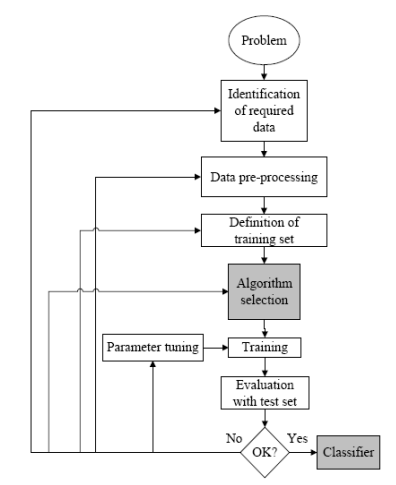
\includegraphics[width=0.5\linewidth]{flowchart.png}
    \centering
    \caption{The Processes of Supervised Machine Learning}
    \label{fig:fig1}
\end{figure}

This work focuses on the classification of ML 
algorithms and determining the most efficient 
algorithm with highest accuracy and precision. As 
well as establishing the performance of different algorithms on large and smaller data sets with a 
view classify them correctly and give insight on 
how to build supervised machine learning models. 

The remaining part of this work is arranged as 
follows: Section 2 presents the literature review 
discussing classification of different supervised 
% learning algorithms; section 3 presents the
% methodology used, section 4 discusses the results of 
% the work while section 5 gives the conclusion and 
% recommendation for further work.

\section{Literature Review} \label{sec2}

\hspace*{1em} According to Ayodele, Taiwo Oladipupo et al. \cite{ref3}, supervised machine learning algorithms that deal more with classification include the following: Linear Classifiers, Logistic Regression, Naïve Bayes Classifier, Perceptron, Support Vector Machine; Quadratic Classifiers, K-Means Clustering, Boosting, Decision Tree, Random Forest (RF); Neural networks, Bayesian Networks, and so on.

\hspace*{1em} The K Nearest Neighbor (kNN) method Zhang et al. \cite{knn} has been widely used in data mining and machine learning applications due to its simple implementation and distinguished performance. However, setting all test data with the same \(k\) value has been proven impractical for real applications. Zhang et al. \cite{knn2} proposed learning a correlation matrix to assign different \(k\) values for different test data points, referred to as the Correlation Matrix kNN (CM-kNN) classification. They utilized a least-squares loss function, a graph Laplacian regularizer, and l1-norm/l2,1-norm regularizers to enhance efficiency. Experiments demonstrated its superior performance in classification, regression, and missing data imputation.

\hspace*{1em} These are among the most recent supervised machine learning techniques Vapnik et al. \cite{svm1}. SVM models revolve around the concept of maximizing the margin on either side of a hyperplane separating two data classes. Kotsiantis et al. \cite{ref2} demonstrated that this approach reduces the expected generalization error effectively.

\hspace*{1em} Logistic regression, as described by Newsom et al. \cite{logistic1}, builds classification models using a multinomial logistic regression approach. It predicts class probabilities, making it suitable for detailed and reliable predictions. Osisanwo et al. \cite{logistic2} highlighted its widespread use in applied statistics and discrete data analysis, noting its robustness and simplicity.

\hspace*{1em} Gradient Boosting is an ensemble learning algorithm used for classification tasks. Monika et al. \cite{xg1} described how it iteratively minimizes a loss function to improve model accuracy. Liew et al. \cite{xg2} emphasized its flexibility, robustness, and high performance, particularly with imbalanced datasets, while highlighting the importance of hyperparameter tuning.

\hspace*{1em} Decision Trees classify instances by sorting them based on feature values. Ayodele et al. \cite{ref2} and Hastie et al. \cite{ref5} discussed their use in data mining and machine learning, noting that decision trees employ pruning techniques for improved accuracy.

\hspace*{1em} Random Forest is an ensemble learning algorithm known for its accuracy and stability. Rigatti et al. \cite{ran1} described its method of building multiple decision trees using bagging and feature randomness to reduce overfitting. It provides insights into feature importance and generalizes well across various datasets.

\hspace*{1em} Gaussian Naive Bayes is a simple yet effective classifier. Isidore Jacob et al. \cite{nv1} and Sebestyen et al. \cite{nv2} highlighted its independence assumption and minimal storage requirements. Despite being less accurate in some scenarios, \citeauthor{nv3} et al. \cite{nv3} found it superior to other methods on benchmark datasets. Its robustness to missing values and ability to work incrementally were further discussed by Domingos et al. \cite{nv4}.

\hspace*{1em} XGBClassifier, based on XGBoost, offers efficient and scalable gradient boosting. Chang et al. \cite{xgb2} detailed its features, including L1/L2 regularization, parallel processing, and missing value handling. Chang et al. \cite{xgb} emphasized its effectiveness in predictive analytics, particularly in large-scale datasets.

\hspace*{1em} Supervised machine learning techniques are applicable across numerous domains. A number of ML application-oriented studies can be found in Setiono et al. \cite{ref6} and Witten et al. \cite{ref7}.

Generally, Decision Tree and Random Forest perform better with multidimensional and continuous features, while logic-based systems excel with discrete features. Isidore Jacob et al. \cite{nv1} noted Naive Bayes's efficiency with minimal storage space and its robustness to missing values. Vapnik et al. \cite{svm1} found that SVMs excel with non-linear relationships and multicollinearity. Meanwhile, Zhang et al. \cite{knn} highlighted k-NN’s sensitivity to irrelevant features, which can impact efficiency.

No single learning algorithm consistently outperforms others across all datasets, as noted by various studies, emphasizing the need for context-specific selection.


% \section{Literature Review} \label{sec2}
% \subsection {Classification of Supervised Learning  Algorithms}
% \hspace*{1em}  According to \cite{ref3}, the supervised machine 
% learning algorithms which deals more with 
% classification includes the following: Linear 
% Classifiers, Logistic Regression, Naïve Bayes 
% Classifier, Perceptron, Support Vector Machine; 
% Quadratic Classifiers, K-Means Clustering, 
% Boosting, Decision Tree, Random Forest (RF); 
% Neural networks, Bayesian Networks and so on. 

% \subsubsection{KNN:} 
% \hspace*{1em} The K Nearest Neighbor (kNN) method \cite{knn} has widely been used in the applications of data mining and machine learning due to its simple implementation and distinguished performance. However, setting all test data with the same k value in the previous kNN methods has been proven to make these methods impractical in real applications. This article proposes to learn a correlation matrix to reconstruct test data points by training data to assign different k values to different test data points, referred to as the Correlation Matrix kNN (CM-kNN for short) classification. Specifically, the least-squares loss function is employed to minimize the reconstruction error to reconstruct each test data point by all training data points. Then, a graph Laplacian regularizer is advocated to preserve the local structure of the data in the reconstruction process. Moreover, an l1-norm regularizer and an l2, 1-norm regularizer are applied to learn different k values for different test data and to result in low sparsity to remove the redundant/noisy feature from the reconstruction process, respectively. Besides for classification tasks, the kNN methods (including our proposed CM-kNN method) are further utilized to regression and missing data imputation. We conducted sets of experiments for illustrating the efficiency, and experimental results showed that the proposed method was more accurate and efficient than existing kNN methods in data-mining applications, such as classification, regression, and missing data imputation. \cite{knn2}


% \subsubsection{Support Vector Machines (SVMs):}
% \hspace{1em}  These are the most recent supervised machine learning technique \cite{svm1}.Support Vector Machine (SVM) 
% models are closelyrelated to classical multilayer 
% perceptron neural networks.SVMs revolve around 
% the notion of a ―margin—either side of a 
% hyperplane that separates two data classes. 
% Maximizing the margin and thereby creating the 
% largest possible distance between the separating 
% hyperplane and the instances on either side of it has 
% been proven to reduce an upper bound on the 
% expected generalisation error. \cite{ref2}

% \subsubsection{Logistic Regression:}
% \hspace{1em}This is a classification
% function that uses class for building and uses a 
% single multinomial logistic regression model with a 
% single estimator. Logistic regression usually states
% where the boundary between the classes exists, also 
% states the class probabilities depend on distance 
% from the boundary, in a specific approach. This 
% moves towards the extremes (0 and 1) more rapidly 
% when data set is larger. These statements about 
% probabilities which make logistic regression more 
% than just a classifier. It makes stronger, more 
% detailed predictions, and can be fit in a different 
% way; but those strong predictions could be wrong.
% Logistic regression is an approach to prediction, like 
% Ordinary Least Squares (OLS) regression. However, 
% with logistic regression, prediction results in a 
% dichotomous outcome.\cite{logistic1} Logistic regression is 
% one of the most commonly used tools for applied 
% statistics and discrete data analysis. Logistic 
% regression is linear interpolation. \cite{logistic2}

% \subsubsection{ GradientBoosting Classifier:}
% \hspace{1em} It is a powerful ensemble machine learning algorithm used for classification tasks. It builds a predictive model in a stage-wise manner by sequentially adding weak learners, typically decision trees, to correct the errors made by the previous models. Each new tree is trained to minimize a loss function, typically the negative gradient of the error with respect to the model's predictions, thereby "boosting" the performance of the ensemble. Gradient Boosting operates by combining the outputs of individual learners, weighted according to their contribution to reducing the error, resulting in a robust and accurate model\cite{xg1}. It uses hyperparameters such as the learning rate (to control the contribution of each tree), the number of estimators (trees), and the maximum depth of trees (to control overfitting) \cite{xg2}. Gradient Boosting Classifier is widely appreciated for its ability to handle complex non-linear relationships, its flexibility in choosing different loss functions, and its high predictive performance, especially in cases of imbalanced datasets. However, it can be computationally intensive and sensitive to hyperparameter tuning, making it important to carefully validate and optimize the model for specific datasets.

% \subsubsection{ Decision Tree:}
% \hspace{1em} These are 
% trees that classify instances by sorting them based 
% on feature values. Each node in a decision tree 
% represents a feature in an instance to be classified, 
% and each branch represents a value that the node can 
% assume. Instances are classified starting at the root 
% node and sorted based on their feature values \cite{ref2}. Decision tree learning, used in data mining and 
% machine learning, uses a decision tree as a 
% predictive model which maps observations about an 
% item to conclusions about the item's target value. 
% More descriptive names for such tree models are 
% classification trees or regression trees \cite{ref5}. Decision tree classifiers usually employ post-pruning 
% techniques that evaluate the performance of decision 
% trees, as they are pruned by using a validation set. 
% Any node can be removed and assigned the most 
% common class of the training instances that are 
% sorted to it. \cite{ref2}

% \subsubsection{Random Forest:}
% \hspace{1em} It is a robust and versatile ensemble learning algorithm used for both classification and regression tasks. It operates by building multiple decision trees during training and combines their predictions to produce accurate and stable results. Each tree is constructed using a random subset of the data, selected with replacement (bagging), and at each split, only a random subset of features is considered. This randomness reduces overfitting and ensures diversity among the trees, enhancing the model's predictive power. For classification, the final output is determined by majority voting among the trees, while for regression, it is based on averaging their predictions. Random Forest is highly effective in handling noisy data, outliers, and high-dimensional datasets, and it provides insights into feature importance, making it useful for feature selection. Although computationally more intensive than simpler models, its ability to generalize well across varied datasets makes it a popular choice in fields like finance, healthcare, and marketing, where accuracy and reliability are critical.\cite{ran1}

% \subsubsection{Gaussian Naive Bayes:}
% \hspace{1em} These
% are very simple Bayesian networks which are 
% composed of directed acyclic graphs with only one 
% parent (representing the unobserved node) and 
% several children (corresponding to observed nodes) 
% with a strong assumption of independence among 
% child nodes in the context of their parent \cite{nv1}. Thus, 
% the independence model (Naive Bayes) is based on 
% estimating \cite{nv2}. Bayes classifiers are usually less 
% accurate that other more sophisticated learning 
% algorithms (such as ANNs).However, \cite{nv3} performed 
% a large-scale comparison of the naive Bayes 
% classifier with state-of-the-art algorithms for 
% decision tree induction, instance-based learning, and 
% rule induction on standard benchmark datasets, and 
% found it to be sometimes superior to the other
% learning schemes, even on datasets with substantial 
% feature dependencies. Bayes classifier has attribute independence problem which was addressed with 
% Averaged One-Dependence Estimators \cite{nv4}.

% \subsubsection{XGBClassifier:}
% \hspace{1em} It is a highly efficient and scalable implementation of the gradient boosting algorithm, provided by the XGBoost library. It builds an ensemble of decision trees in a stage-wise manner, where each tree corrects the errors of the previous ones by minimizing a gradient-based loss function \cite{xgb2}. XGBClassifier includes advanced features like regularization (L1 and L2) to prevent overfitting, built-in handling of missing values, and parallel processing to improve computational efficiency \cite{xgb}.  It also supports techniques like column sampling and distributed computing, making it suitable for handling large-scale and high-dimensional datasets. With its ability to provide fast training, robust predictions, and feature importance analysis, XGBClassifier is widely used in machine learning competitions, predictive analytics, and real-world applications in domains such as finance, healthcare, and e-commerce.


% \subsection{Features of Machine Learning Algorithms}
% \hspace{1em}Supervised machine learning techniques are 
% applicable in numerous domains. A number of 
% Machine Learning (ML) application oriented papers 
% can be found in \cite{ref6}, \cite{ref7}.

% Generally, Decison Tree and Random Forest tend to 
% perform much better when dealing with multidimensions and continuous features. On the other 
% hand, logic-based systems tend to perform better 
% when dealing with discrete/categorical features. For Naive Bayes, SVMs, a large sample size is required in order to achieve its maximum prediction accuracy.

% There is general agreement that k-NN is very 
% sensitive to irrelevant features: this characteristic 
% can be explained by the way the algorithm works. 
% Moreover, the presence of irrelevant features can 
% make neural network training very inefficient, even
% impractical.Most decision tree algorithms cannot 
% perform well with problems that require diagonal 
% partitioning. The division of the instance space is 
% orthogonal to the axis of one variable and parallel to 
% all other axes. Therefore, the resulting regions after 
% partitioning are all hyperrectangles. The SVMs perform well when multi-collinearity is 
% present and a nonlinear relationship exists between 
% the input and output features.

% Naive Bayes (NB) requires little storage space 
% during both the training and classification stages: the 
% strict minimum is the memory needed to store the 
% prior and conditional probabilities. The basic kNN 
% algorithm uses a great deal of storage space for the 
% training phase, and its execution space is at least as 
% big as its training space. On the contrary, for all 
% non-lazy learners, execution space is usually much 
% smaller than training space, since the resulting 
% classifier is usually a highly condensed summary of 
% the data. Moreover, Naive Bayes and the kNN can 
% be easily used as incremental learners whereas rule 
% algorithms cannot. Naive Bayes is naturally robust 
% to missing values since these are simply ignored in 
% computing probabilities and hence have no impact 
% on the final decision. On the contrary, kNN require complete records to do their work.

% Finally, Decision Trees and NB generally have 
% different operational profiles, when one is very 
% accurate the other is not and vice versa. On the 
% contrary, decision trees and rule classifiers have a 
% similar operational profile. SVM has 
% also a similar operational profile. No single learning 
% algorithm can uniformly outperform other 
% algorithms over all datasets.

% %
\section{Dataset Description}
The UCI Heart Disease dataset \cite{dataset} is a well-known collection of data used for predicting the presence of heart disease in patients. It contains 14 attributes, including demographic information, clinical measurements, and diagnostic results, such as age, sex, chest pain type, resting blood pressure, cholesterol levels, and maximum heart rate achieved. The dataset is used to train machine learning models for classification tasks, where the goal is to predict whether a patient has heart disease based on these features. The dataset is frequently used for benchmarking various algorithms and understanding the relationships between different cardiovascular risk factors \cite{dataset}.
\subsection{Age}
\textbf{Description:} 
Age is the patient’s age in years, one of the most critical factors for cardiovascular diseases. \\
\textit{Key insights:}
\begin{itemize}
    \item Age-related arterial stiffening leads to hypertension.
    \item Risk increases sharply after 45 years in men and 55 years in women.
    \item Younger patients with heart issues often have hereditary or congenital conditions.
\end{itemize}
\textbf{Graph Analysis:} 
The distribution is nearly normal, centered around 54 years. The slight negative skew indicates a higher concentration of older individuals. This implies that middle-aged and elderly individuals dominate the dataset, aligning with the expected demographic for heart disease prevalence. The alignment of the mean, median, and mode emphasizes the symmetric nature of the data.

\subsection{Sex}
\textbf{Description:} 
Sex is defined as the biological sex of the patient (Male/Female). Gender differences influence heart disease risk. \\
\textit{Key insights:}
\begin{itemize}
    \item Men are at higher risk before age 50 due to higher LDL levels and lifestyle factors.
    \item Post-menopause, women’s risk increases due to estrogen decline.
    \item Symptoms like atypical pain in women often delay diagnosis.
\end{itemize}
\textbf{Graph Analysis:} 
The dataset is heavily male-dominated, with males constituting about 79\% of the samples. This imbalance highlights a potential bias in the dataset, and models trained on it might not generalize well for females. Additionally, this distribution might reflect real-world trends, as men are often at higher risk for certain types of heart diseases.

\subsection{Chest Pain Type (CP)}
\textbf{Description:} 
Chest pain type describes the nature of chest pain: typical angina, atypical angina, non-anginal, or asymptomatic. It is a crucial diagnostic feature. \\
\textit{Key insights:}
\begin{itemize}
    \item Typical angina indicates reduced blood flow due to coronary artery disease.
    \item Atypical or non-anginal pain might point to non-cardiac causes.
    \item Asymptomatic patients are concerning due to silent ischemia risks.
\end{itemize}
\textbf{Graph Analysis:} 
Over half of the cases are asymptomatic (54\%), which is a common scenario in heart diseases. Non-anginal and atypical angina follow, with typical angina being the least common. This pattern, coupled with variations across genders, emphasizes the importance of chest pain type in diagnosis and analysis.

\subsection{Resting Blood Pressure (Trestbps)}
\textbf{Description:} 
Resting blood pressure measures the systolic pressure in mmHg. High values indicate hypertension, a key heart disease risk factor. \\
\textit{Key insights:}
\begin{itemize}
    \item Blood pressure $\geq$140 mmHg is linked to atherosclerosis and left ventricular hypertrophy.
    \item Managing blood pressure can significantly reduce cardiovascular risk.
\end{itemize}
\textbf{Graph Analysis:} 
The average resting blood pressure is 132 mmHg, slightly above the normal range (120 mmHg). The slight negative skew indicates some individuals with significantly higher blood pressure. Such variations emphasize hypertension's role as a risk factor for heart diseases.

\subsection{Serum Cholesterol (Chol)}
\textbf{Description:} 
Serum cholesterol measures total cholesterol (mg/dL). Elevated levels increase the risk of plaque buildup, causing arterial narrowing. \\
\textit{Key insights:}
\begin{itemize}
    \item LDL contributes to blockages, while HDL protects against plaque formation.
    \item Levels $\geq$240 mg/dL are linked to higher risks of strokes and heart attacks.
\end{itemize}
\textbf{Graph Analysis:} 
The average cholesterol level is 199 mg/dL, with a few extreme values creating a long tail. Most individuals cluster near the average, but the outliers suggest a subset of the population at higher cardiovascular risk due to elevated cholesterol.

\subsection{Fasting Blood Sugar (FBS)}
\textbf{Description:} 
FBS measures fasting blood sugar, with levels $>$120 mg/dL indicating diabetes risk. High glucose levels are linked to cardiovascular complications. \\
\textit{Key insights:}
\begin{itemize}
    \item Diabetes accelerates atherosclerosis and damages blood vessels.
    \item Early detection is crucial for preventing severe outcomes.
\end{itemize}
\textbf{Graph Analysis:} 
Most individuals (approximately 83\%) have normal fasting blood sugar levels (False). The small proportion with elevated levels indicates potential comorbidities like diabetes, which are critical in heart disease prognosis.

\subsection{Resting ECG (Restecg)}
\textbf{Description:} 
Resting ECG records the heart's electrical activity, identifying conditions like ischemia or past infarctions. \\
\textit{Key insights:}
\begin{itemize}
    \item Normal results are a baseline for further testing.
    \item Abnormalities provide evidence for severe cardiac conditions.
\end{itemize}
\textbf{Graph Analysis:} 
About 60\% of the samples show normal ECG results, while the remaining indicate abnormalities such as left ventricular hypertrophy or ST-T wave changes. This distribution suggests a mix of normal and at-risk cardiac conditions in the dataset.

\subsection{Maximum Heart Rate Achieved (Thalach)}
\textbf{Description:} 
Thalach measures the highest heart rate during exercise, reflecting cardiovascular fitness. \\
\textit{Key insights:}
\begin{itemize}
    \item Lower heart rates can indicate blockages or reduced cardiac function.
    \item Exercise tolerance is an indirect marker of heart health.
\end{itemize}
\textbf{Graph Analysis:} 
Most individuals achieve a maximum heart rate close to 138 bpm, indicating good cardiovascular fitness for a significant portion of the population. Outliers on the lower side suggest individuals with compromised heart function.

\subsection{ST Depression (Oldpeak)}
\textbf{Description:} 
ST depression measures the difference in the ST segment during exercise, with higher values indicating myocardial ischemia. \\
\textit{Key insights:}
\begin{itemize}
    \item A crucial diagnostic tool for coronary artery disease.
    \item Guides decisions for further interventions like angiography.
\end{itemize}
\textbf{Graph Analysis:} 
Values near zero, indicating minimal ST depression during exercise. However, the few higher values reflect individuals at higher risk for ischemia, emphasizing its importance as a diagnostic metric.

\subsection{Slope of ST Segment (Slope)}
\textbf{Description:} 
The slope during peak exercise (upsloping, flat, or downsloping) reflects blood flow. \\
\textit{Key insights:}
\begin{itemize}
    \item Flat or downsloping slopes suggest reduced oxygen supply to the heart.
\end{itemize}
\textbf{Graph Analysis:} 
The flat slope is the most frequent, indicating ischemia in a majority of cases. The upsloping and downsloping categories offer additional diagnostic insights, often correlated with exercise-induced stress test results.

\subsection{Number of Major Vessels (CA)}
\textbf{Description:} 
The number of major vessels visible through fluoroscopy (0-3). Lower numbers indicate more severe blockages. \\
\textit{Key insights:}
\begin{itemize}
    \item Fewer vessels detected correlate with worse arterial health.
\end{itemize}
\textbf{Graph Analysis:} 
Most individuals (181 samples) have zero major vessels detected, which is indicative of less severe conditions. The distribution emphasizes the progression of heart disease severity based on the number of vessels affected.

\subsection{Thalassemia (Thal)}
\textbf{Description:} 
A blood disorder affecting oxygen transport, categorized as normal, fixed defect, or reversible defect. \\
\textit{Key insights:}
\begin{itemize}
    \item Fixed defects indicate permanent damage.
    \item Reversible defects suggest treatable ischemia.
\end{itemize}
\textbf{Graph Analysis:} 
The "normal" category is the most frequent, followed by fixed and reversible defects. Fixed defects indicate permanent damage, while reversible defects suggest ischemia that could potentially be treated.

\section{Data Processing}
\begin{enumerate}
    \item \textbf{Dataset Loading:}
    \begin{itemize}
        \item The dataset was loaded in CSV file from UCI Heart Disease Dataset \cite{dataset}.
        \item Initial inspection using \texttt{df.info()} and \texttt{df.describe()} provided insights into data types, missing values, and statistical distributions.
    \end{itemize}
    
    \item \textbf{Exploratory Data Analysis (EDA):}
    \begin{itemize}
        \item \textbf{Distribution Analysis:} Visualized each column to understand its distribution using histograms and boxplots.
        \item \textbf{Correlation Analysis:} Created a heatmap to understand correlations between numerical columns and identify relationships.
        \item \textbf{Categorical Feature Analysis:} Examined value counts and proportions for categorical variables like \texttt{sex}, \texttt{cp} (chest pain type), and \texttt{thal}.
    \end{itemize}

    \item \textbf{Irrelevant Column Removal:}
    \begin{itemize}
        \item Dropped columns that did not add value to the prediction, such as:
        \begin{itemize}
            \item \texttt{id} (row identifier)
            \item \texttt{dataset} (data source information)
        \end{itemize}
    \end{itemize}
    
    \item \textbf{Handling Missing Values:}
    \begin{itemize}
        \item \textbf{Categorical Variables:}
        \begin{itemize}
            \item \textbf{Columns Affected:} \texttt{slope}, \texttt{thal}, \texttt{exang}, \texttt{restecg}, \texttt{fbs}.
            \item \textbf{Imputation Strategy:} Used the \textbf{most frequent value (mode)} to fill missing values.
        \end{itemize}
        \item \textbf{Numerical Variables:}
        \begin{itemize}
            \item \textbf{Columns Affected:} \texttt{trestbps} (resting blood pressure), \texttt{chol} (cholesterol), \texttt{thalch} (maximum heart rate), \texttt{oldpeak} (ST depression).
            \item \textbf{Imputation Strategy:} Filled missing values using the \textbf{mean}.
        \end{itemize}
        \item \textbf{High-Missingness Columns:}
        \begin{itemize}
            \item \texttt{ca} (number of major vessels): Included in categorical imputation due to its potential relevance.
        \end{itemize}
    \end{itemize}

    \item \textbf{Outlier Detection and Treatment:}
    \begin{itemize}
        \item \textbf{Outlier Identification:}
        \begin{itemize}
            \item Inspected boxplots for numerical variables: \texttt{oldpeak}, \texttt{thalch}, \texttt{chol}, and \texttt{trestbps}.
            \item Detected extreme values deviating significantly from normal distributions.
        \end{itemize}
    \end{itemize}

        
        \item \textbf{Outlier Detection and Treatment:}
    \begin{itemize}
        \item \textbf{Outlier Identification:}
        \begin{itemize}
            \item Outliers were detected by visualizing boxplots for numerical variables: \texttt{oldpeak}, \texttt{thalch}, \texttt{chol}, and \texttt{trestbps}. Boxplots provide a graphical summary of data distributions and help visually identify potential outliers. Outliers are typically shown as points beyond the "whiskers" of the boxplot.
            \item Mathematically, an outlier is defined as any data point that lies outside a specific range, which is determined using the Interquartile Range (IQR). 
        \end{itemize}
        
        \item \textbf{Outlier Handling Strategy:}
        \begin{itemize}
            \item \textbf{Interquartile Range (IQR) Method:} The IQR is the range between the first quartile (\( Q1 \)) and the third quartile (\( Q3 \)) of the data. The formula to compute the IQR is:
            \[
            \text{IQR} = Q3 - Q1
            \]
            \item Once the IQR is calculated, outliers are identified using the following bounds:
            \begin{align*}
                \text{Lower Bound} &= Q1 - 1.5 \times \text{IQR} \\
                \text{Upper Bound} &= Q3 + 1.5 \times \text{IQR}
            \end{align*}
            Any data point that falls below the lower bound or above the upper bound is considered an outlier.
            
            \item \textbf{Outlier Capping:} Outliers that lie outside these bounds are not removed, but rather capped to the nearest valid value (either the lower or upper bound). This method prevents extreme outliers from unduly affecting the model while retaining all observations for analysis.
            \item \textbf{Exceptions:} For certain variables, such as the \texttt{age} column, large values were not capped because they are realistic and within the expected range for the dataset. The rationale is that extreme ages (e.g., very old individuals) may not be outliers in the context of medical data and should be retained for analysis.
        \end{itemize}
    \end{itemize}


    \item \textbf{Encoding Categorical Data:}
    \begin{itemize}
        \item \textbf{Nominal Variables:}
        \begin{itemize}
            \item Columns such as \texttt{sex}, \texttt{cp}, \texttt{restecg}, \texttt{exang}, \texttt{thal}, and \texttt{fbs} were \textbf{one-hot encoded}.
        \end{itemize}
        \item \textbf{Ordinal Variables:}
        \begin{itemize}
            \item \texttt{slope}: Ordinally encoded to preserve the order of categories.
        \end{itemize}
    \end{itemize}

    \item \textbf{Feature Engineering:}
    \begin{itemize}
        \item \textbf{Derived Features:}
        \begin{itemize}
            \item \texttt{bp\_to\_chol\_ratio}: This feature represents the ratio between resting blood pressure (\texttt{trestbps}) and cholesterol (\texttt{chol}). The rationale behind creating this feature is to capture a relationship between two cardiovascular risk factors. It is believed that the balance between blood pressure and cholesterol can provide additional insight into an individual’s health risk.
            \item \texttt{age\_to\_max\_hr}: This feature calculates the ratio between a person’s age (\texttt{age}) and their maximum heart rate (\texttt{thalch}). This derived feature is intended to highlight how age influences an individual's heart performance. As age increases, a decrease in maximum heart rate is expected, so this ratio can offer insight into the cardiovascular fitness of an individual relative to their age. All of these has been done here. By this we get two new features.
        \end{itemize}
        
        
        \item \textbf{Feature Selection:}
        \begin{itemize}
            \item \texttt{id} (row identifier): This column was dropped because it is a unique identifier for each row, providing no meaningful information for model prediction. Including it would have no impact on the outcome of the analysis or model training.
            \item \texttt{dataset} (data source information): This column was also dropped as it pertains to the source of the dataset and does not contribute directly to the analysis or predictive modeling process.
        \end{itemize}
        
        \item \textbf{Reorganization:}
        \begin{itemize}
            \item The columns were reorganized to prioritize more relevant features. In this case, \texttt{age} (an important predictor), engineered features (\texttt{bp\_to\_chol\_ratio} and \texttt{age\_to\_max\_hr}), and the encoded variables (such as one-hot encoded columns) were placed at the beginning of the dataset. This reordering helps streamline the feature set and makes it easier to manage when applying machine learning models.
        \end{itemize}
    \end{itemize}


    \item \textbf{Automated Preprocessing Pipeline:}
    \begin{itemize}
        \item \textbf{Pipeline Components:}
        \begin{itemize}
            \item Defined separate transformation pipelines for:
            \begin{itemize}
                \item \textbf{Numerical Columns:} Mean imputation and scaling using \texttt{StandardScaler}.
                \item \textbf{Categorical Columns:} Mode imputation, one-hot encoding, and ordinal encoding.
            \end{itemize}
        \end{itemize}
        \item \textbf{Final Processed Dataset:}
        \begin{itemize}
            \item Unified preprocessing using \texttt{Pipeline} and \texttt{ColumnTransformer}.
            \item Ensured consistent transformations for training and testing datasets.
        \end{itemize}
    \end{itemize}

    \item \textbf{Scaling and Final Adjustments:}
    \begin{itemize}
        \item \textbf{Feature Scaling:}
        \begin{itemize}
            \item Applied \texttt{StandardScaler} to scale numerical features for magnitude consistency.
        \end{itemize}
        \item \textbf{Final Dataset Size and Structure:}
        \begin{itemize}
            \item The processed dataset contained 920 rows and 25 columns after transformations and feature engineering.
            \item Included engineered features and encoded variables, with missing values and outliers resolved.
        \end{itemize}
    \end{itemize}
\end{enumerate}











\section{Research Methodology}
The research methodology employed a variety of machine learning algorithms to analyze the dataset and predict the target variable effectively. Each model was carefully chosen and implemented based on its strengths and compatibility with the problem at hand. The dataset \cite{dataset} originally consisted of 16 attributes, including \texttt{id} (a unique identifier) and \texttt{dataset} (study location). These two attributes were excluded during preprocessing as they do not contribute meaningful information to the prediction of heart disease. Removing non-informative features like \texttt{id} helps reduce noise, simplify the dataset, and improve model performance by focusing only on clinically relevant attributes. Consequently, the final dataset used for analysis contained 14 attributes.
 Below is a detailed explanation of the algorithms used and their justification.

\textbf{Algorithms Used:}
The study utilized K-Nearest Neighbors (KNN) as one of the baseline models. KNN works by comparing a test point to its nearest neighbors in the feature space and predicting based on majority voting. It is simple yet effective, especially when the dataset is small and the relationship between features is intuitive.

The Support Vector Machine (SVM) was applied with a linear kernel, ideal for datasets where the decision boundary is linear. SVM creates an optimal hyperplane to separate classes, making it powerful for high-dimensional feature spaces. Its ability to handle outliers and complex classification tasks makes it a suitable choice.

Logistic Regression was employed for its statistical robustness and ability to predict binary outcomes. This model is well-suited for datasets where the relationship between features and the target variable is approximately linear. Logistic regression also provides probabilistic predictions, which are valuable for interpreting results.

Advanced ensemble methods like the Gradient Boosting Classifier and Random Forest were included in the study. Gradient Boosting sequentially builds models to minimize errors, capturing non-linear relationships and improving predictive performance. Random Forest, on the other hand, leverages an ensemble of decision trees to enhance accuracy and reduce the risk of overfitting. This method is particularly useful when the dataset has a mix of categorical and continuous variables.

A Decision Tree model was also tested for its simplicity and interpretability. Decision trees split the dataset based on feature thresholds, making the decision-making process highly transparent. This model is effective for exploratory analysis and for understanding feature importance.

The Gaussian Naive Bayes classifier was applied to handle continuous features. This model assumes a Gaussian distribution of features and provides a computationally efficient method for classification. It is particularly useful for datasets with overlapping feature distributions.

Finally, the XGBoost (Extreme Gradient Boosting) algorithm was included due to its efficiency and high performance in classification tasks. XGBoost uses gradient boosting but optimizes it for speed and accuracy, making it a preferred choice for structured data and competitions.

Justification:
Each model was chosen with specific problem characteristics in mind. For example, KNN was suitable for establishing a baseline because of its simplicity and lack of assumptions about the data distribution. Meanwhile, SVM was chosen for its ability to handle high-dimensional spaces and robustness to outliers.

Logistic Regression served as a foundational model due to its simplicity and interpretability, while Gradient Boosting and Random Forest were employed to capture complex, non-linear patterns and reduce overfitting through ensemble methods. The inclusion of Decision Trees provided valuable insights into the feature space, which is crucial for understanding the factors influencing predictions.

Gaussian Naive Bayes was particularly effective for features with a Gaussian-like distribution, ensuring computational efficiency. The use of XGBoost allowed for optimized performance, as it combines gradient boosting with regularization techniques to prevent overfitting while enhancing predictive power.

All models were evaluated on performance metrics such as precision, recall, F1-score, accuracy, and confusion matrices to ensure their appropriateness and reliability for the dataset. This rigorous approach ensured that the research findings were robust and well-supported by the chosen methodologies. The below table  represents the number of cases in each class of the predicting heart disease column.


\begin{table}[h] 
\label{table:heart}
\csvautotabular{files/num_coun.csv} %define this function
\caption{Heart Disease Class Counts}  % Table heading
\end{table}

\section{Implementation}

\subsection{Tools and Libraries}
The project was implemented using Python, leveraging several libraries for data manipulation, visualization, and machine learning. The primary libraries used include:
\begin{itemize}
    \item \textbf{Pandas} and \textbf{NumPy}: These were used for data manipulation and preprocessing tasks, such as handling missing values, computing statistics, and preparing data for model training \cite{pandas2020gettingstarted, numpy2020gettingstarted}.
    \item \textbf{Matplotlib}, \textbf{Seaborn}, and \textbf{Plotly}: These libraries were utilized for data visualization, enabling the creation of insightful plots such as histograms, scatter plots, and interactive visualizations \cite{hunter2007matplotlib, seaborn2020gettingstarted, plotly2020gettingstarted}.
    \item \textbf{Scikit-learn}: This served as the primary machine learning library, providing tools for splitting the dataset, model training, and evaluation using metrics like accuracy, precision, recall, F1-score, and ROC-AUC \cite{pedregosa2011scikit}.
    \item \textbf{Joblib}: This was used for saving and loading trained models, ensuring reusability and efficiency during deployment \cite{joblib2020documentation}.
\end{itemize}

\subsection{Dataset Loading and Preprocessing}
The dataset, related to heart disease, was loaded from an external URL using Pandas and inspected to understand its structure. The following steps were performed:
\begin{itemize}
    \item The size, data types, and basic statistics of the dataset were assessed using methods such as \texttt{info()}, \texttt{shape}, and \texttt{describe()}.
    \item Missing values were identified in certain columns, such as cholesterol (\texttt{chol}) and resting blood pressure (\texttt{trestbps}), and handled appropriately during preprocessing.
\end{itemize}

\subsection{Parameters}
While specific hyperparameter tuning details were not explicitly defined, the model's performance was optimized by evaluating metrics such as accuracy, precision, recall, and ROC-AUC. These metrics guided model adjustments and ensured robustness.

\subsection{Training Process}
The implementation process consisted of the following steps:
\begin{enumerate}
    \item \textbf{Data Splitting}: The dataset was divided into independent variables (features) and the dependent variable (\texttt{num}), representing the target. A portion of the data (20\%) was reserved for testing to ensure unbiased evaluation.
    \item \textbf{Model Training}: Classification models were trained on the training data using Scikit-learn. Metrics such as accuracy, precision, recall, F1-score, and ROC-AUC were computed to assess model performance.
\end{enumerate}

\subsection{Evaluation}
The models were evaluated on the testing set using performance metrics like confusion matrix, ROC curve, and classification report. This ensured that the trained model generalized well to unseen data, validating its effectiveness.


\section{Result}
In this section, we present the evaluation results for multiple machine learning models applied to the classification task. Each model's performance is assessed using confusion matrices, which provide insight into the types of errors made by the model, including false positives and false negatives. In addition to the confusion matrices, we also discuss the general behavior of the models, highlight potential areas for improvement, and emphasize the importance of considering additional metrics such as precision, recall, and F1-score for a more comprehensive assessment.


A confusion matrix is a fundamental tool in classification problems used to evaluate the performance of a model. Mathematically, it is a square matrix that compares the predicted labels against the actual labels for a classification problem, typically with two classes (binary classification), but it can be extended to multi-class problems. The matrix consists of four key components for binary classification: True Positive (TP), False Positive (FP), True Negative (TN), and False Negative (FN).

\[
\begin{pmatrix}
    TP & FP \\
    FN & TN
\end{pmatrix}
\]

\begin{itemize}
    \item \textbf{True Positives (TP)}: Instances where both the predicted label and the actual label are positive.
    \item \textbf{False Positives (FP)}: Instances where the predicted label is positive, but the actual label is negative.
    \item \textbf{True Negatives (TN)}: Instances where both the predicted label and the actual label are negative.
    \item \textbf{False Negatives (FN)}: Instances where the predicted label is negative, but the actual label is positive.
\end{itemize}

These values are used to calculate various performance metrics, such as accuracy, precision, recall, and the F1-score, which are essential for understanding how well the model is performing. For instance, accuracy is defined as

\[
\text{Accuracy} = \frac{TP + TN}{TP + FP + TN + FN}
\]

while precision and recall are derived from

\[
\text{Precision} = \frac{TP}{TP + FP}, \quad \text{Recall} = \frac{TP}{TP + FN}
\]

The confusion matrix is crucial because it provides insight into the types of errors the model is making, helping to diagnose areas for improvement \cite{confusion_matrix_ref}.


\textbf{Evaluation by Confusion Matrix:} \\
The KNN model demonstrates a relatively balanced performance in classifying both positive and negative cases. Although it performs reasonably well overall, there are instances of misclassification in both directions, including false positives and false negatives. While the confusion matrix suggests that KNN is effective for this problem, a deeper analysis of precision and recall would be beneficial to further understand the model's performance, particularly in handling specific types of errors \autoref{fig:image1}.

The performance of the SVM model is comparable to that of KNN, with similar patterns of misclassification. Although the model achieves a good overall performance, the confusion matrix suggests that there may be a slight bias towards one class. However, further analysis is required to confirm whether SVM's predictions are biased. While the model is reasonable, like KNN, there is room for improvement \autoref{fig:image2}. 

Logistic regression outperforms both KNN and SVM in terms of overall accuracy, suggesting stronger predictive capabilities. While there are still some instances of false positives and false negatives, these errors are fewer compared to the previous models. Given its high accuracy, logistic regression is considered a strong candidate for this classification task. Nonetheless, it would be prudent to compare it with other models to determine its relative performance \autoref{fig:image3}.

Gradient Boosting demonstrates the highest accuracy among all models tested, with very few false positives and false negatives, indicating strong predictive power. However, the possibility of overfitting must be considered, as the model performs exceptionally well on the test data. A comparison of training and testing performance is necessary to assess whether the model generalizes well to unseen data \autoref{fig:image4}.

The Decision Tree model performs well but falls slightly behind Gradient Boosting in terms of accuracy. While Decision Trees are interpretable, they are also prone to overfitting, which warrants careful evaluation of the model's performance on unseen data. Despite this, its interpretability makes it a valuable tool, especially when transparency in decision-making is important \autoref{fig:image5}.

Random Forest exhibits excellent performance, comparable to that of Gradient Boosting, with high accuracy and robustness. Unlike a single Decision Tree, Random Forest is less susceptible to overfitting, making it a reliable model. However, further comparison with Gradient Boosting is necessary to identify the most optimal model \autoref{fig:image6}.

The Naive Bayes model provides decent performance, but its accuracy generally lags behind that of tree-based models and logistic regression. Its primary advantages lie in its simplicity and computational efficiency, making it a suitable candidate for baseline performance. However, for higher accuracy, other models are likely preferable \autoref{fig:image7}.

XGBoost is another model that shows high accuracy, similar to Gradient Boosting and Random Forest. It benefits from advanced features such as regularization and handling missing values, which enhance its performance. While it is a top contender, further comparison with Gradient Boosting and Random Forest is needed to determine which model performs best overall \autoref{fig:image8}.


\begin{figure}[htbp]
\centering
\begin{minipage}{0.45\textwidth}
    \centering
    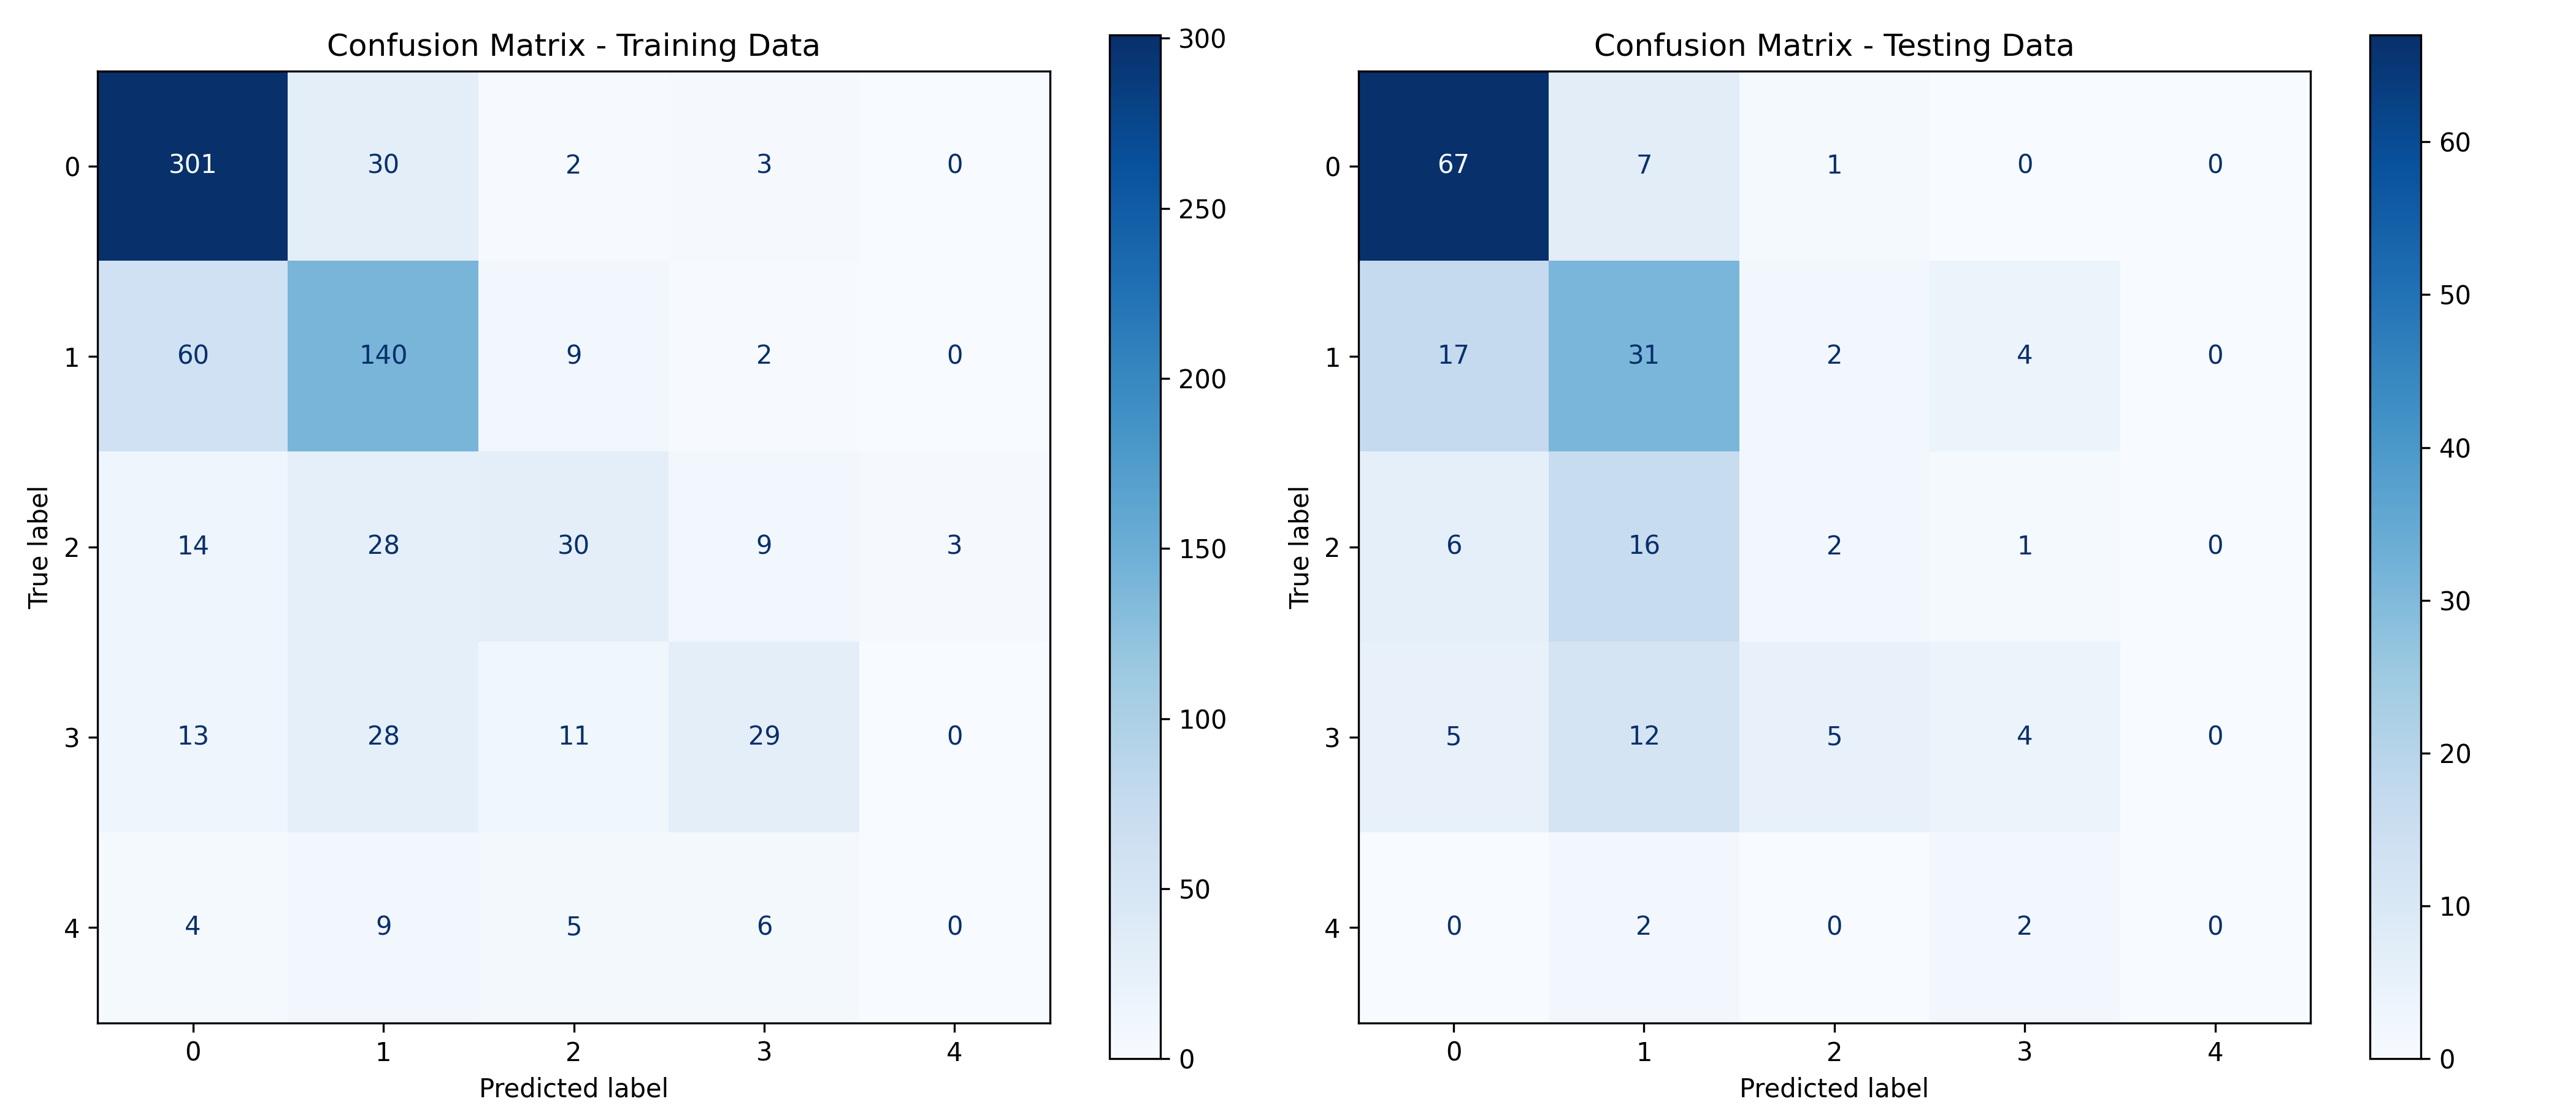
\includegraphics[width=\linewidth]{files/knn1.png}
    \subcaption{KNN Classifier}
    \label{fig:image1}
\end{minipage}%
\hfill
\begin{minipage}{0.45\textwidth}
    \centering
    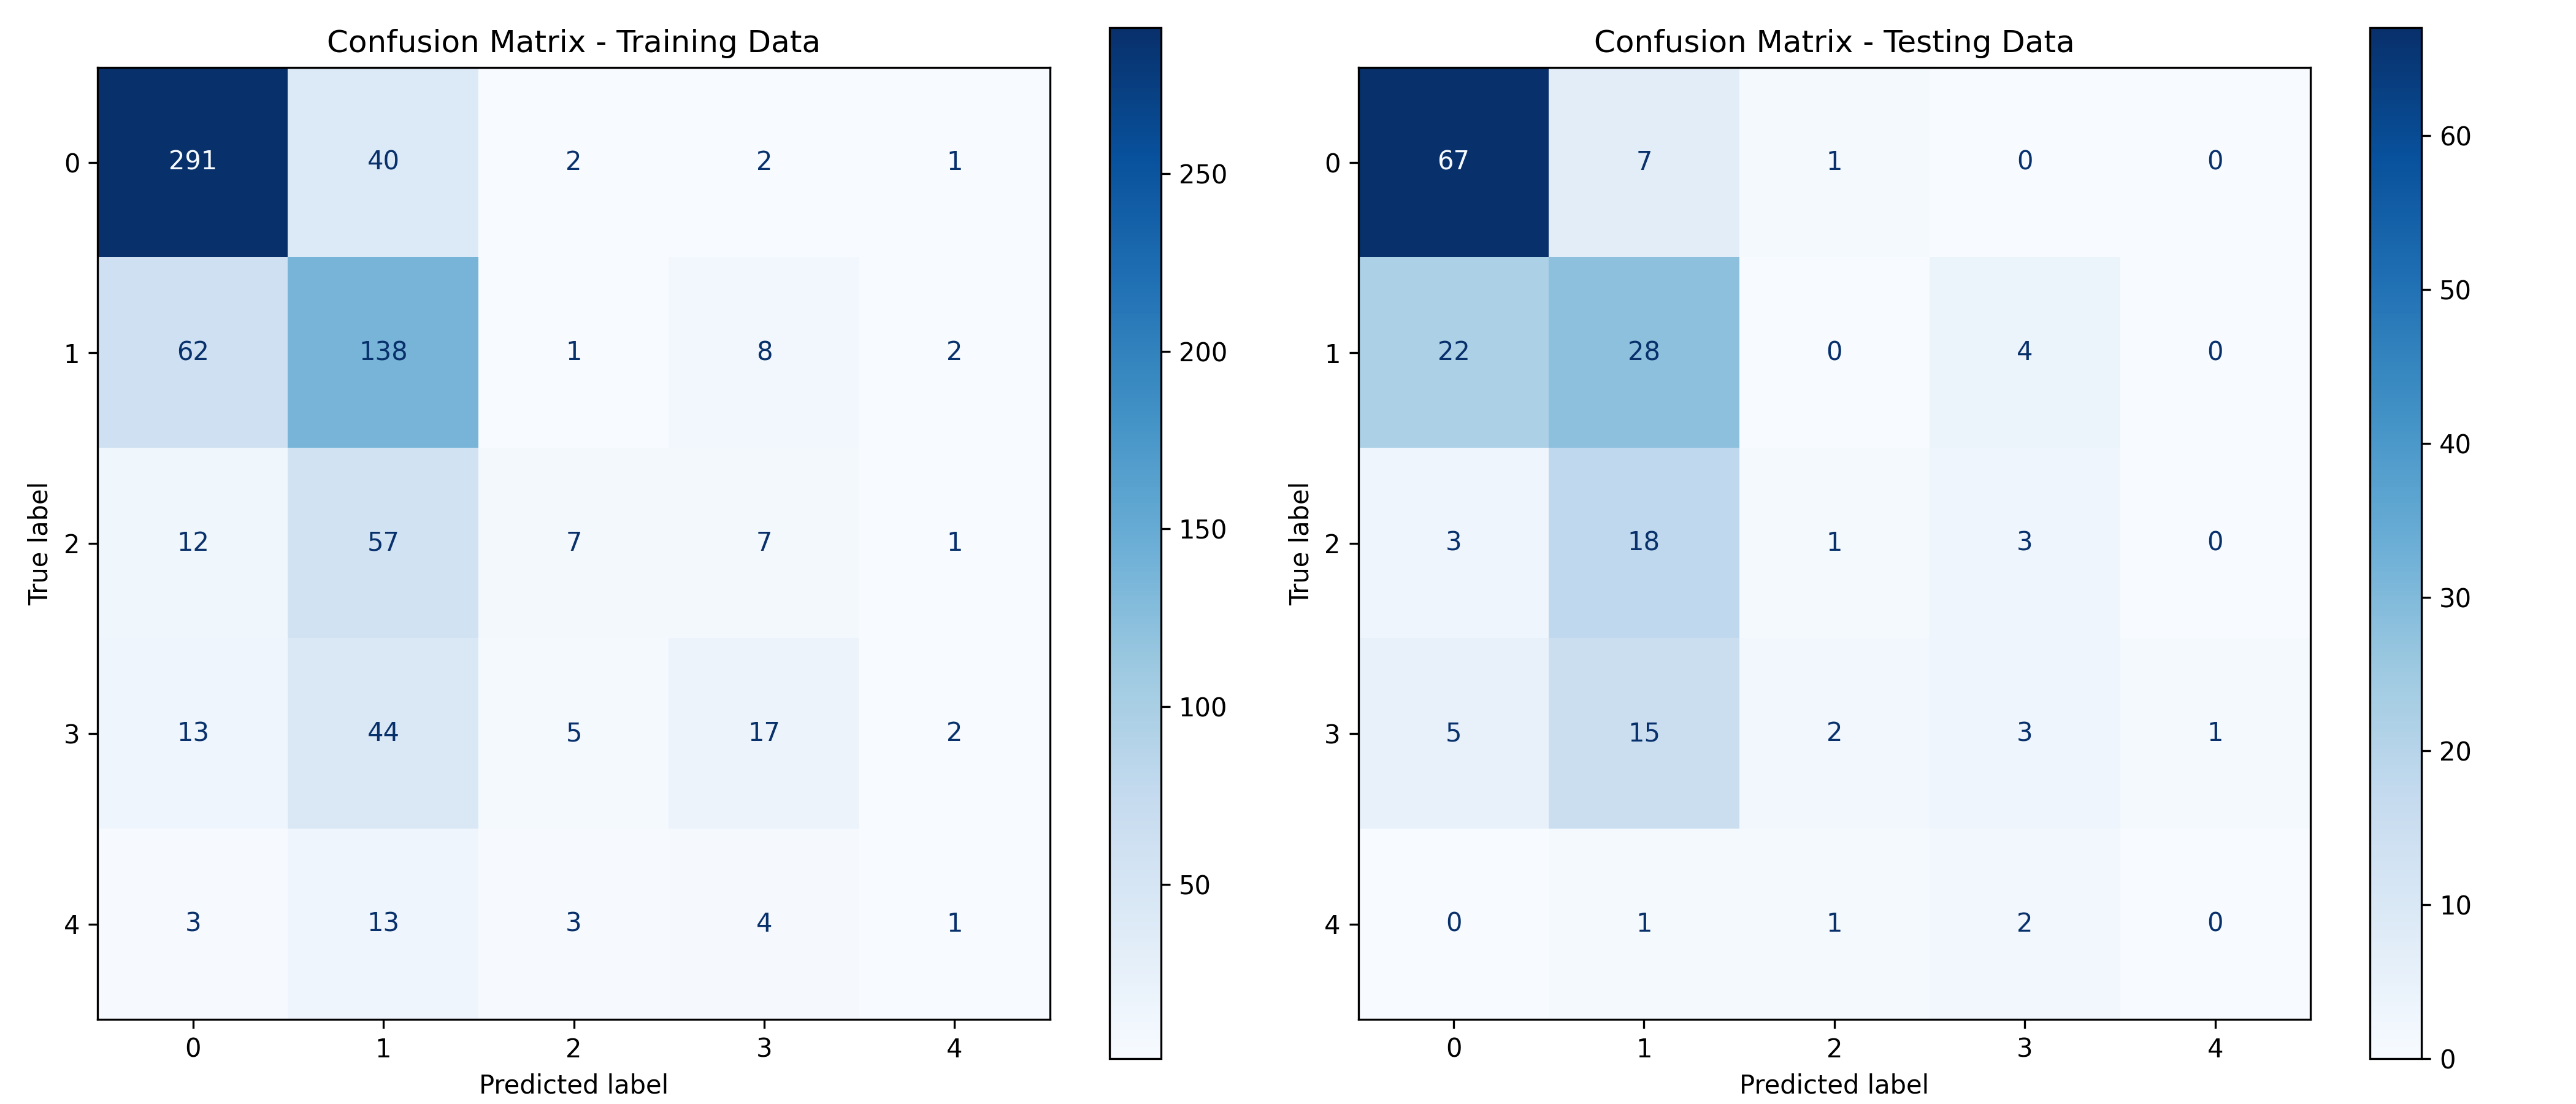
\includegraphics[width=\linewidth]{files/svm1.png}
    \subcaption{SVM Classifier}
    \label{fig:image2}
\end{minipage}

\vspace{1em}

\begin{minipage}{0.45\textwidth}
    \centering
    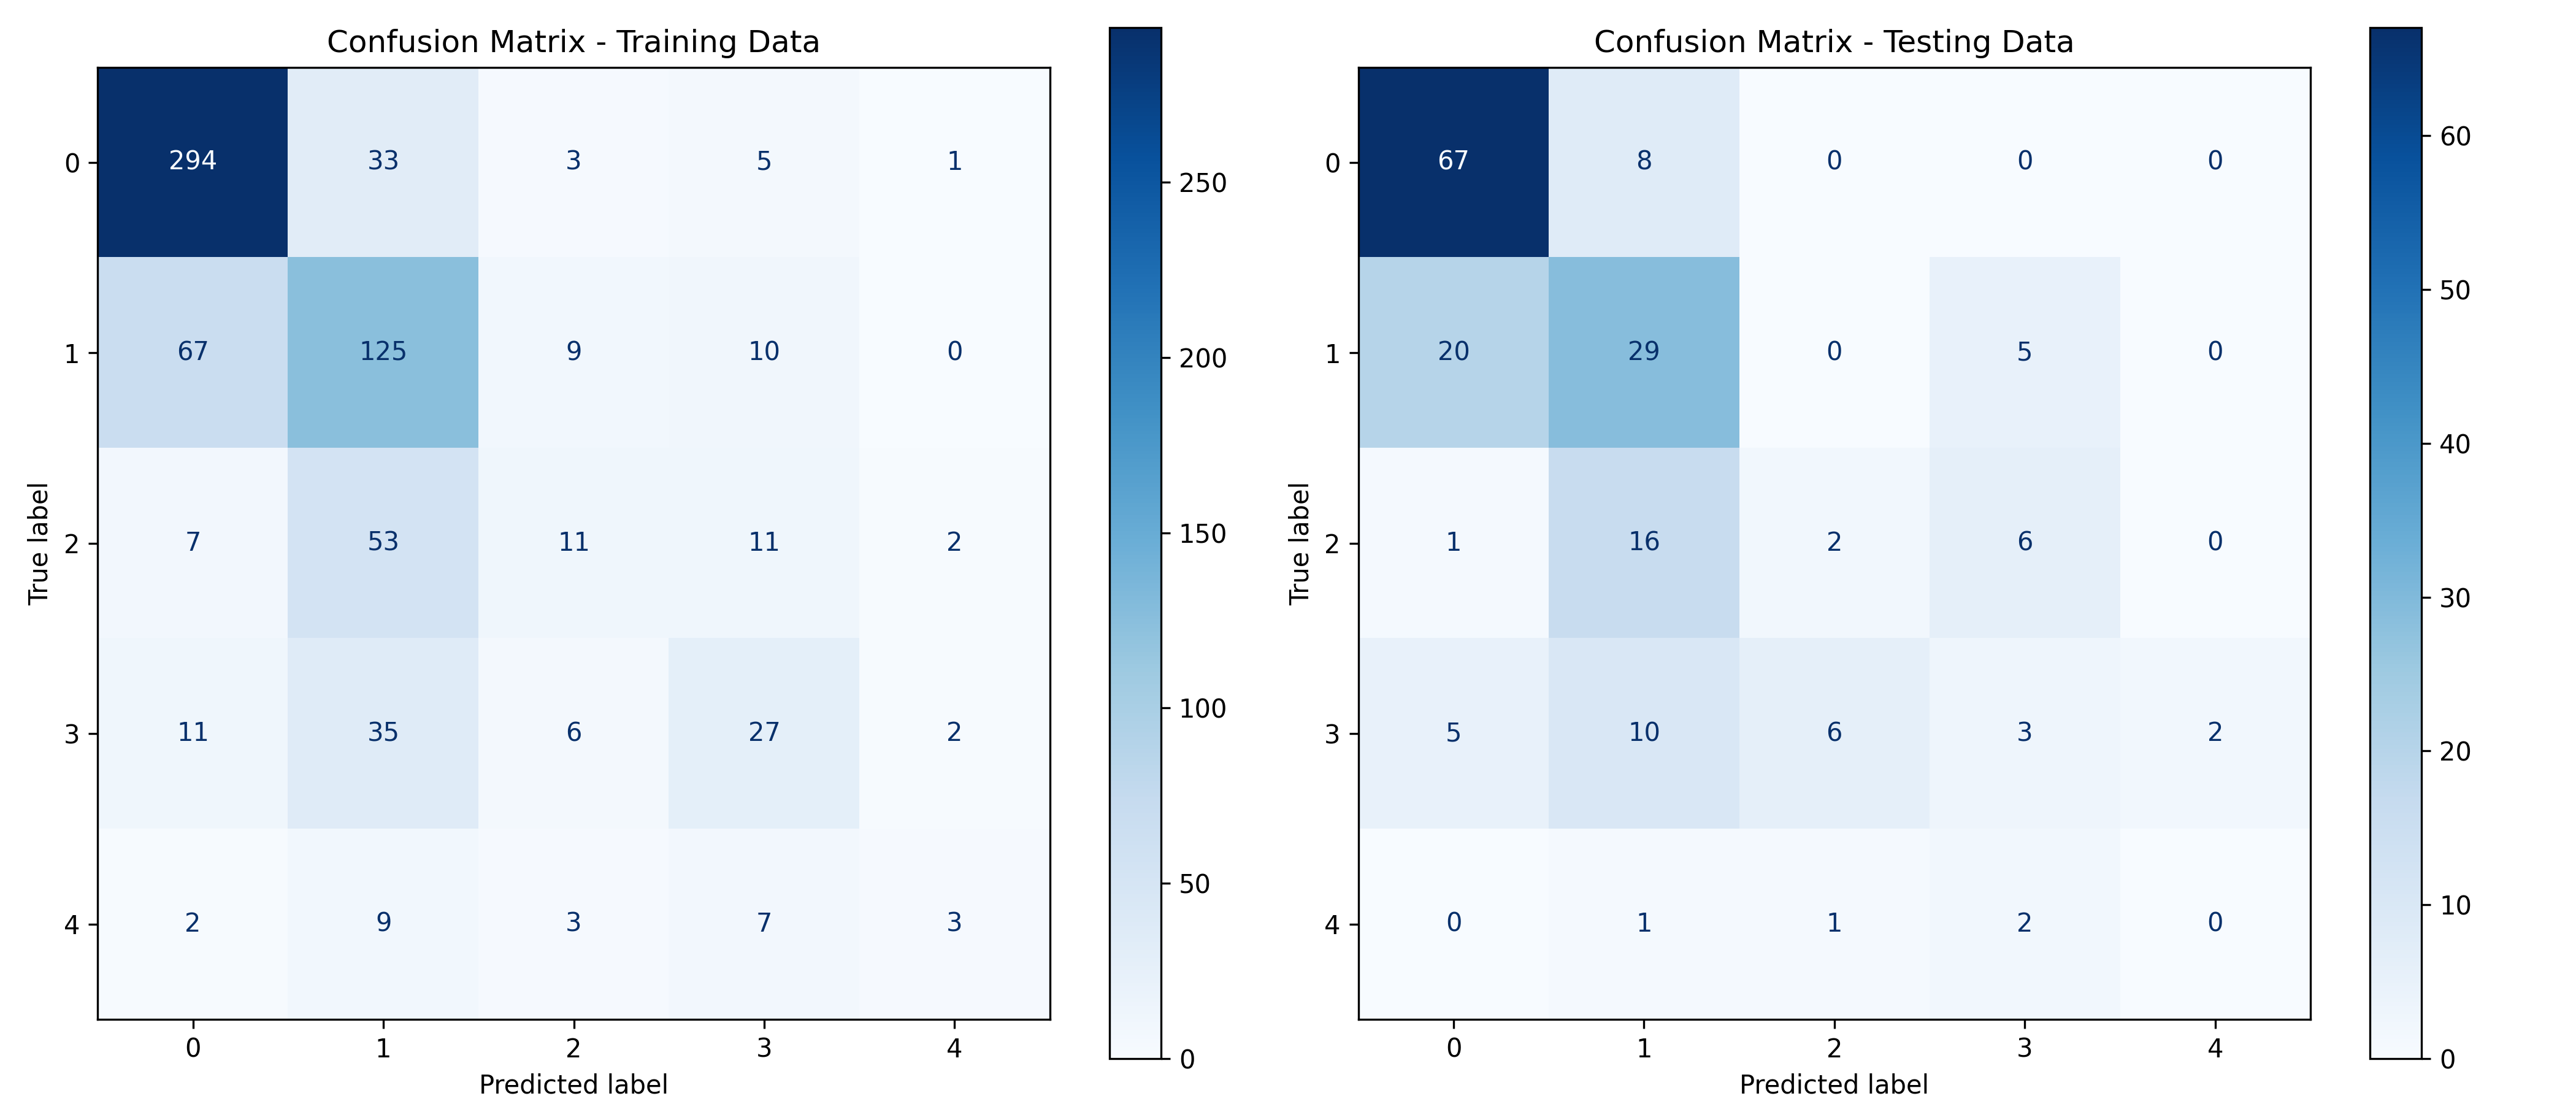
\includegraphics[width=\linewidth]{files/logis1.png}
    \subcaption{Logistic Regression Classifier}
    \label{fig:image3}
\end{minipage}%
\hfill
\begin{minipage}{0.45\textwidth}
    \centering
    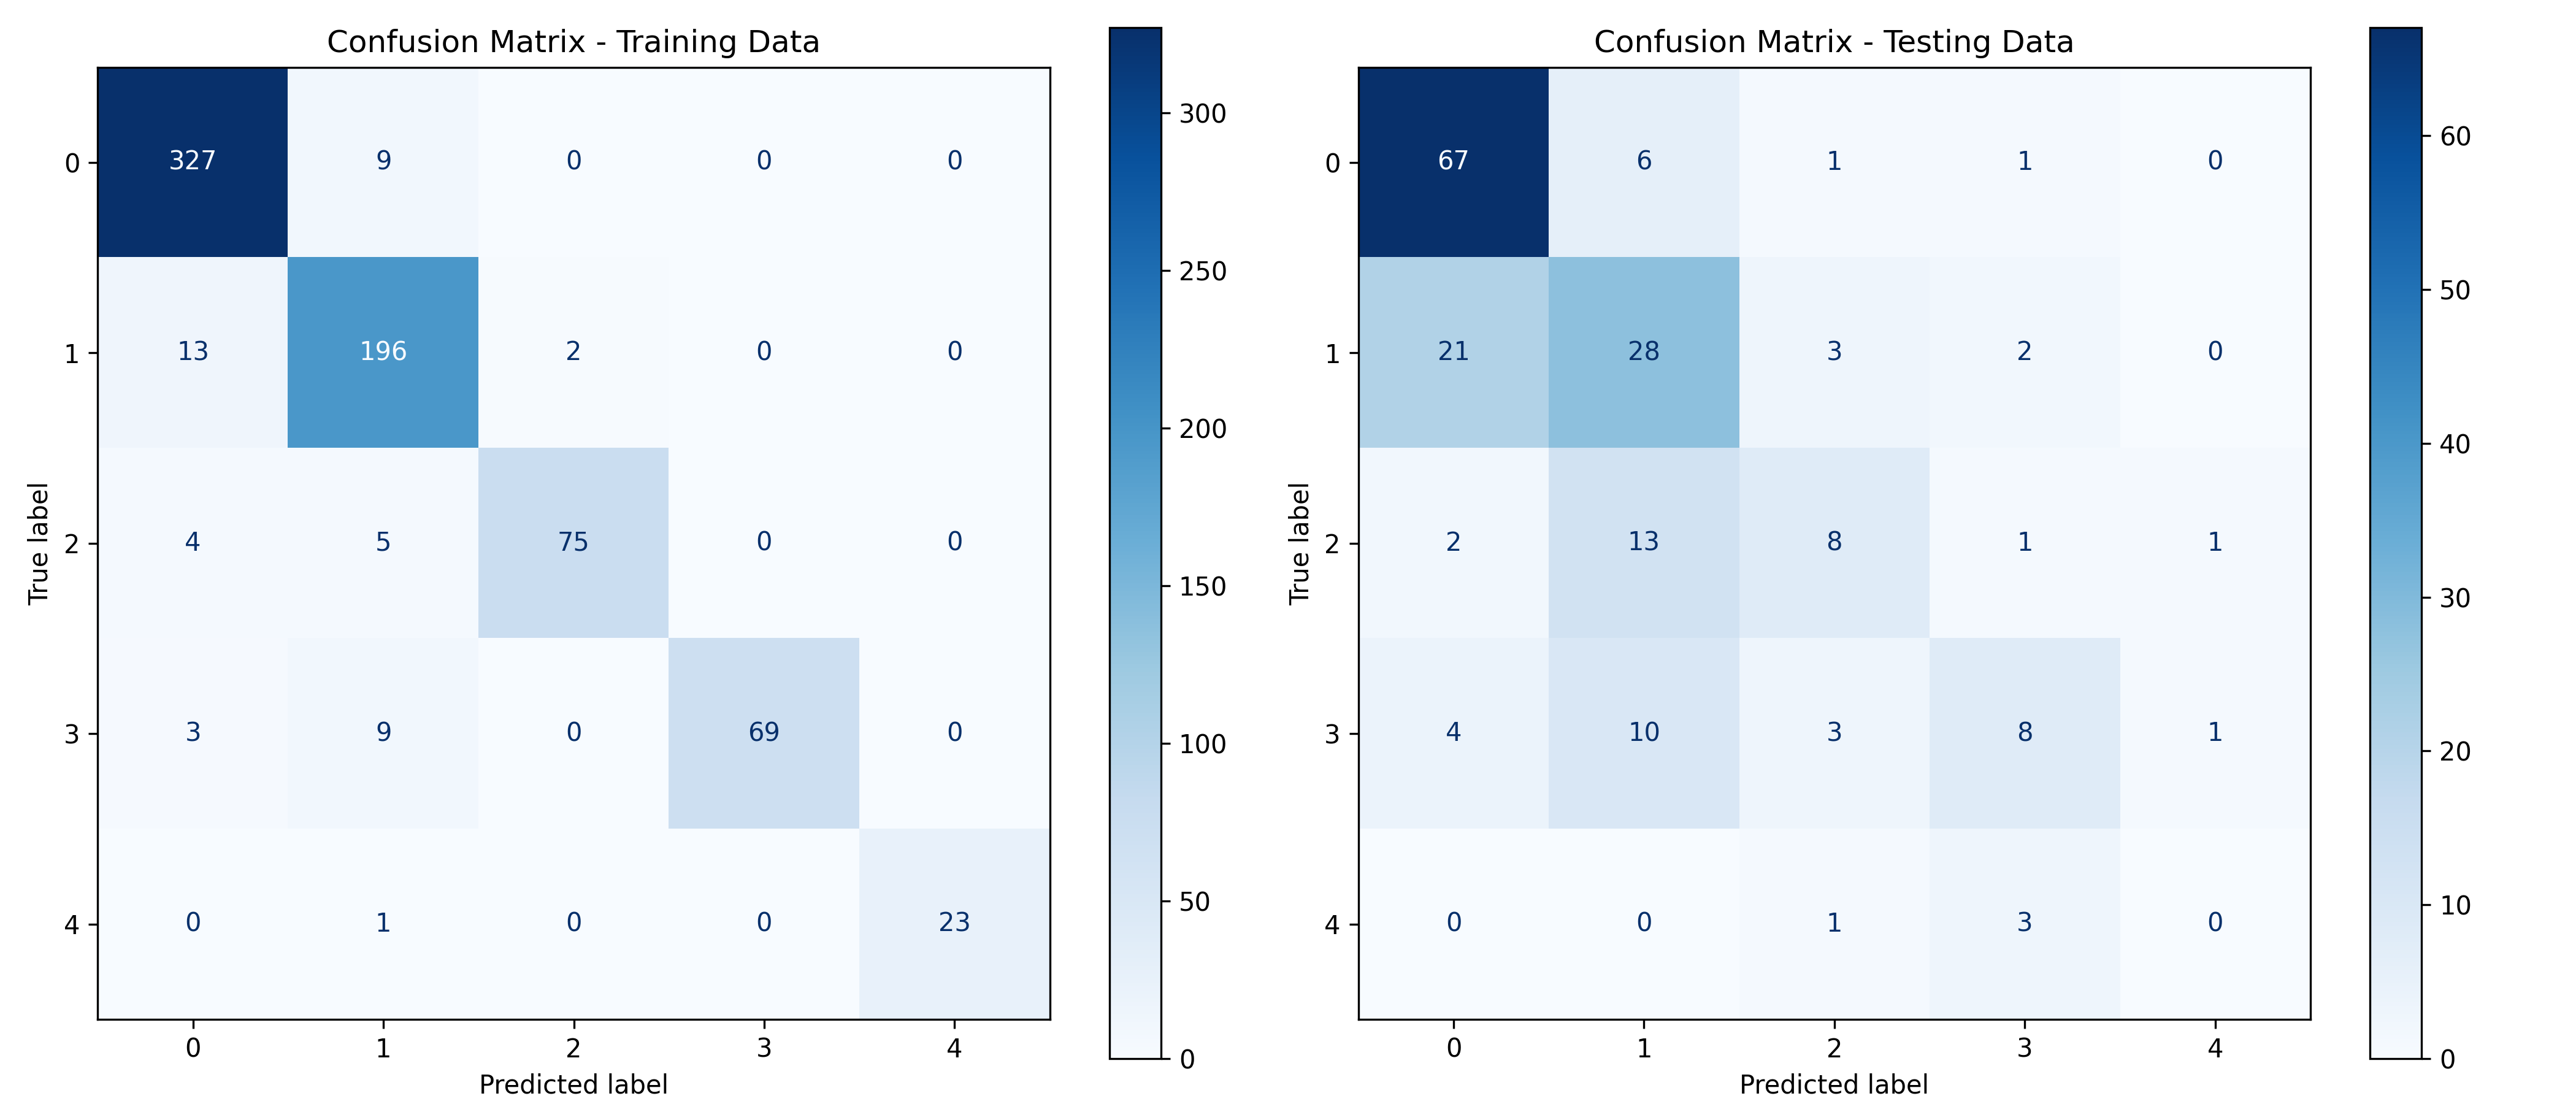
\includegraphics[width=\linewidth]{files/Gradient1.png}
    \subcaption{Gradient Boosting Classifier}
    \label{fig:image4}
\end{minipage}

\vspace{1em}

\begin{minipage}{0.45\textwidth}
    \centering
    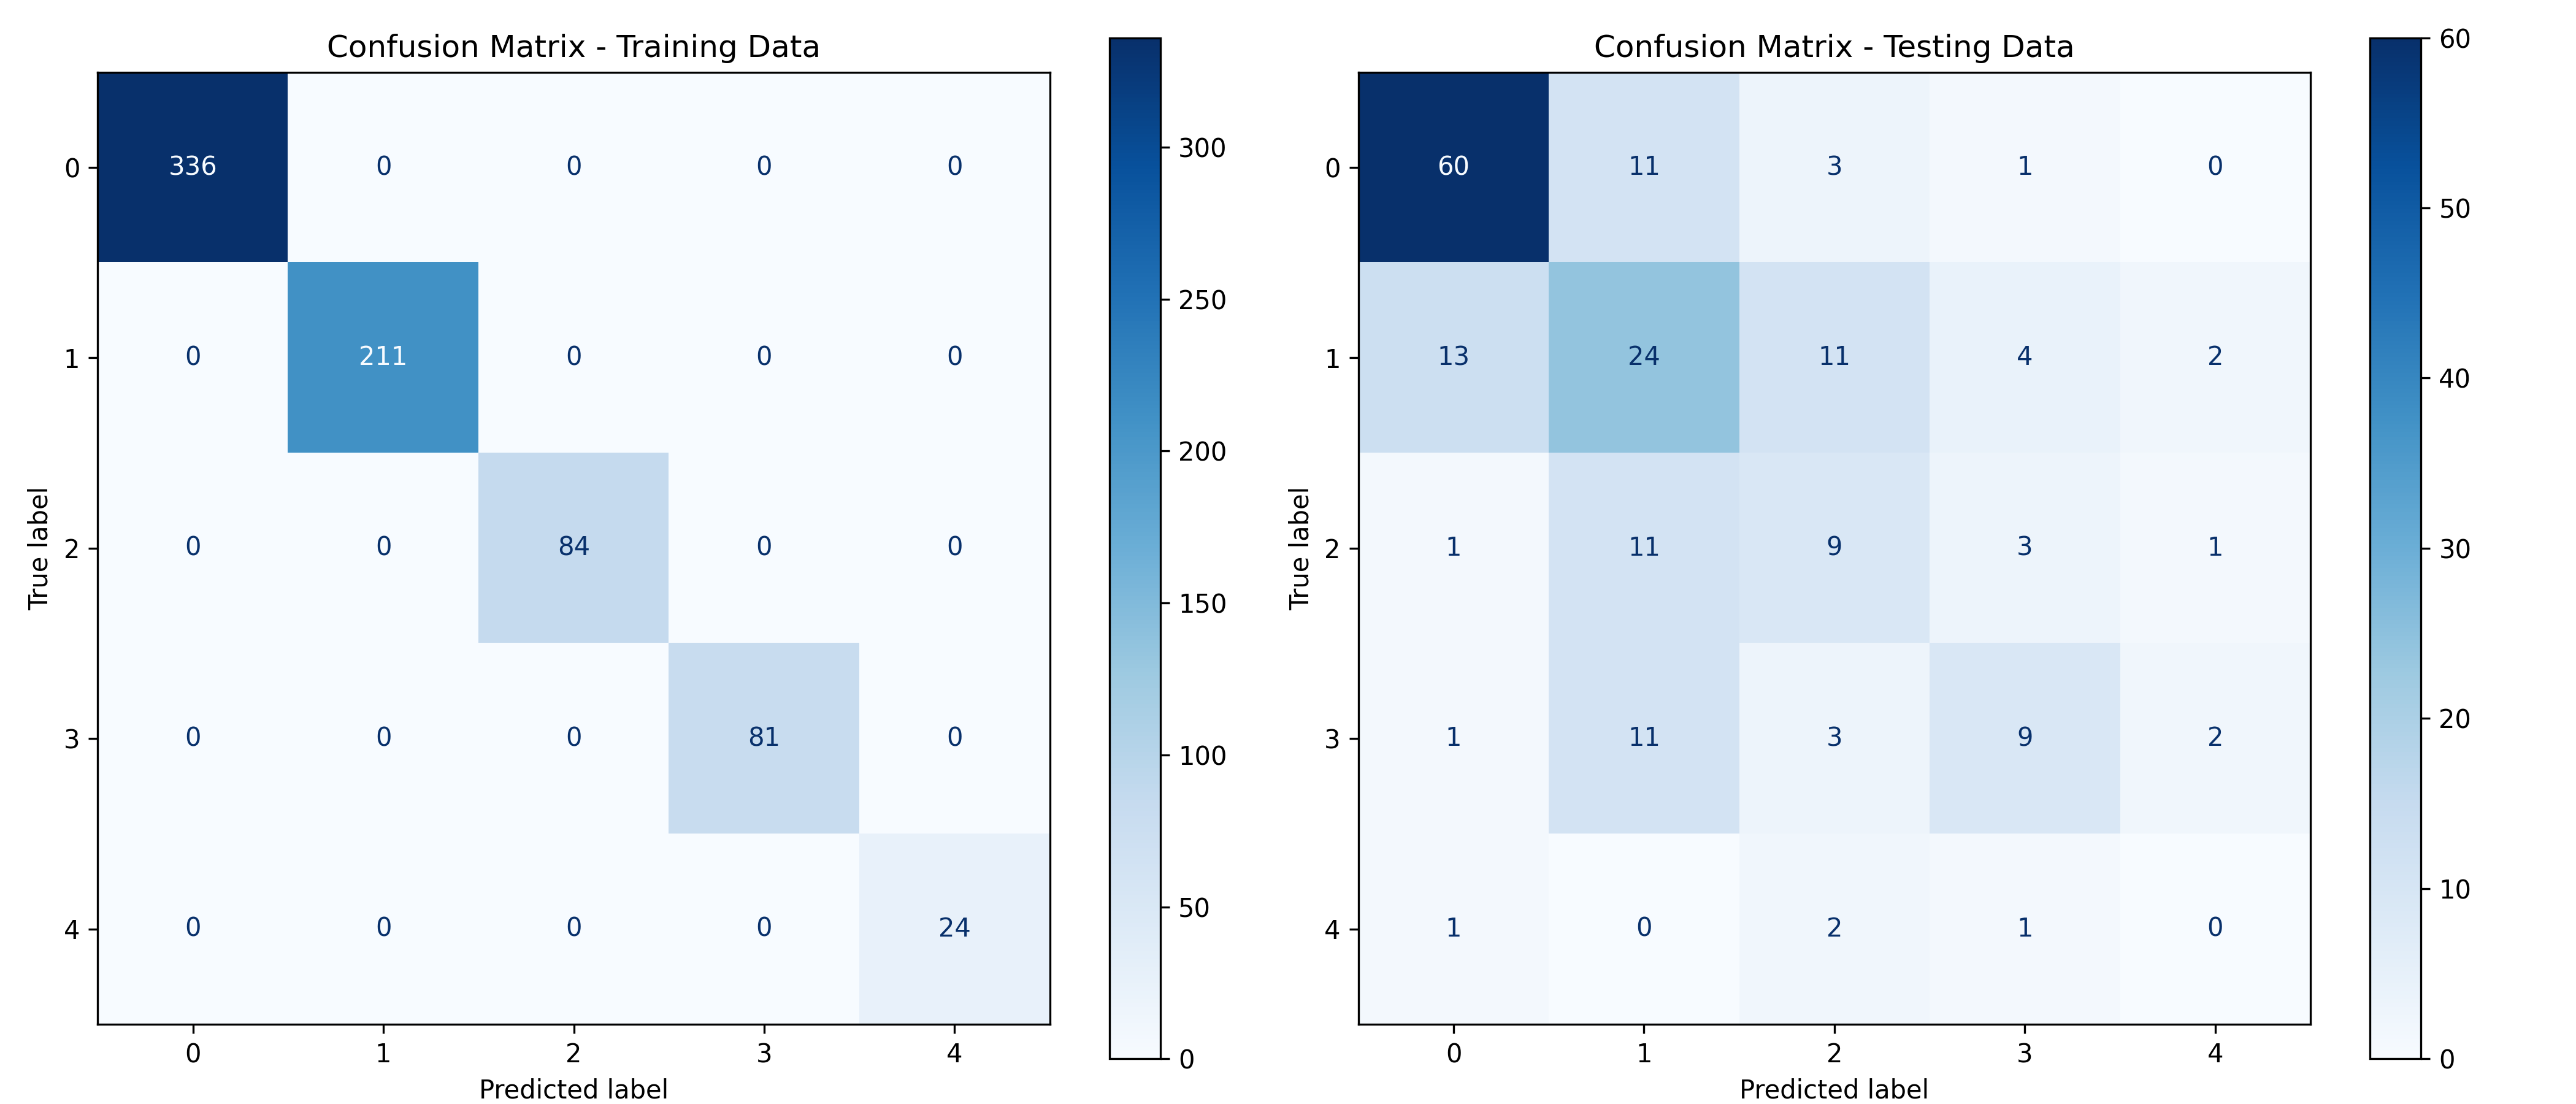
\includegraphics[width=\linewidth]{files/Decision1.png}
    \subcaption{Decision Tree Classifier}
    \label{fig:image5}
\end{minipage}%
\hfill
\begin{minipage}{0.45\textwidth}
    \centering
    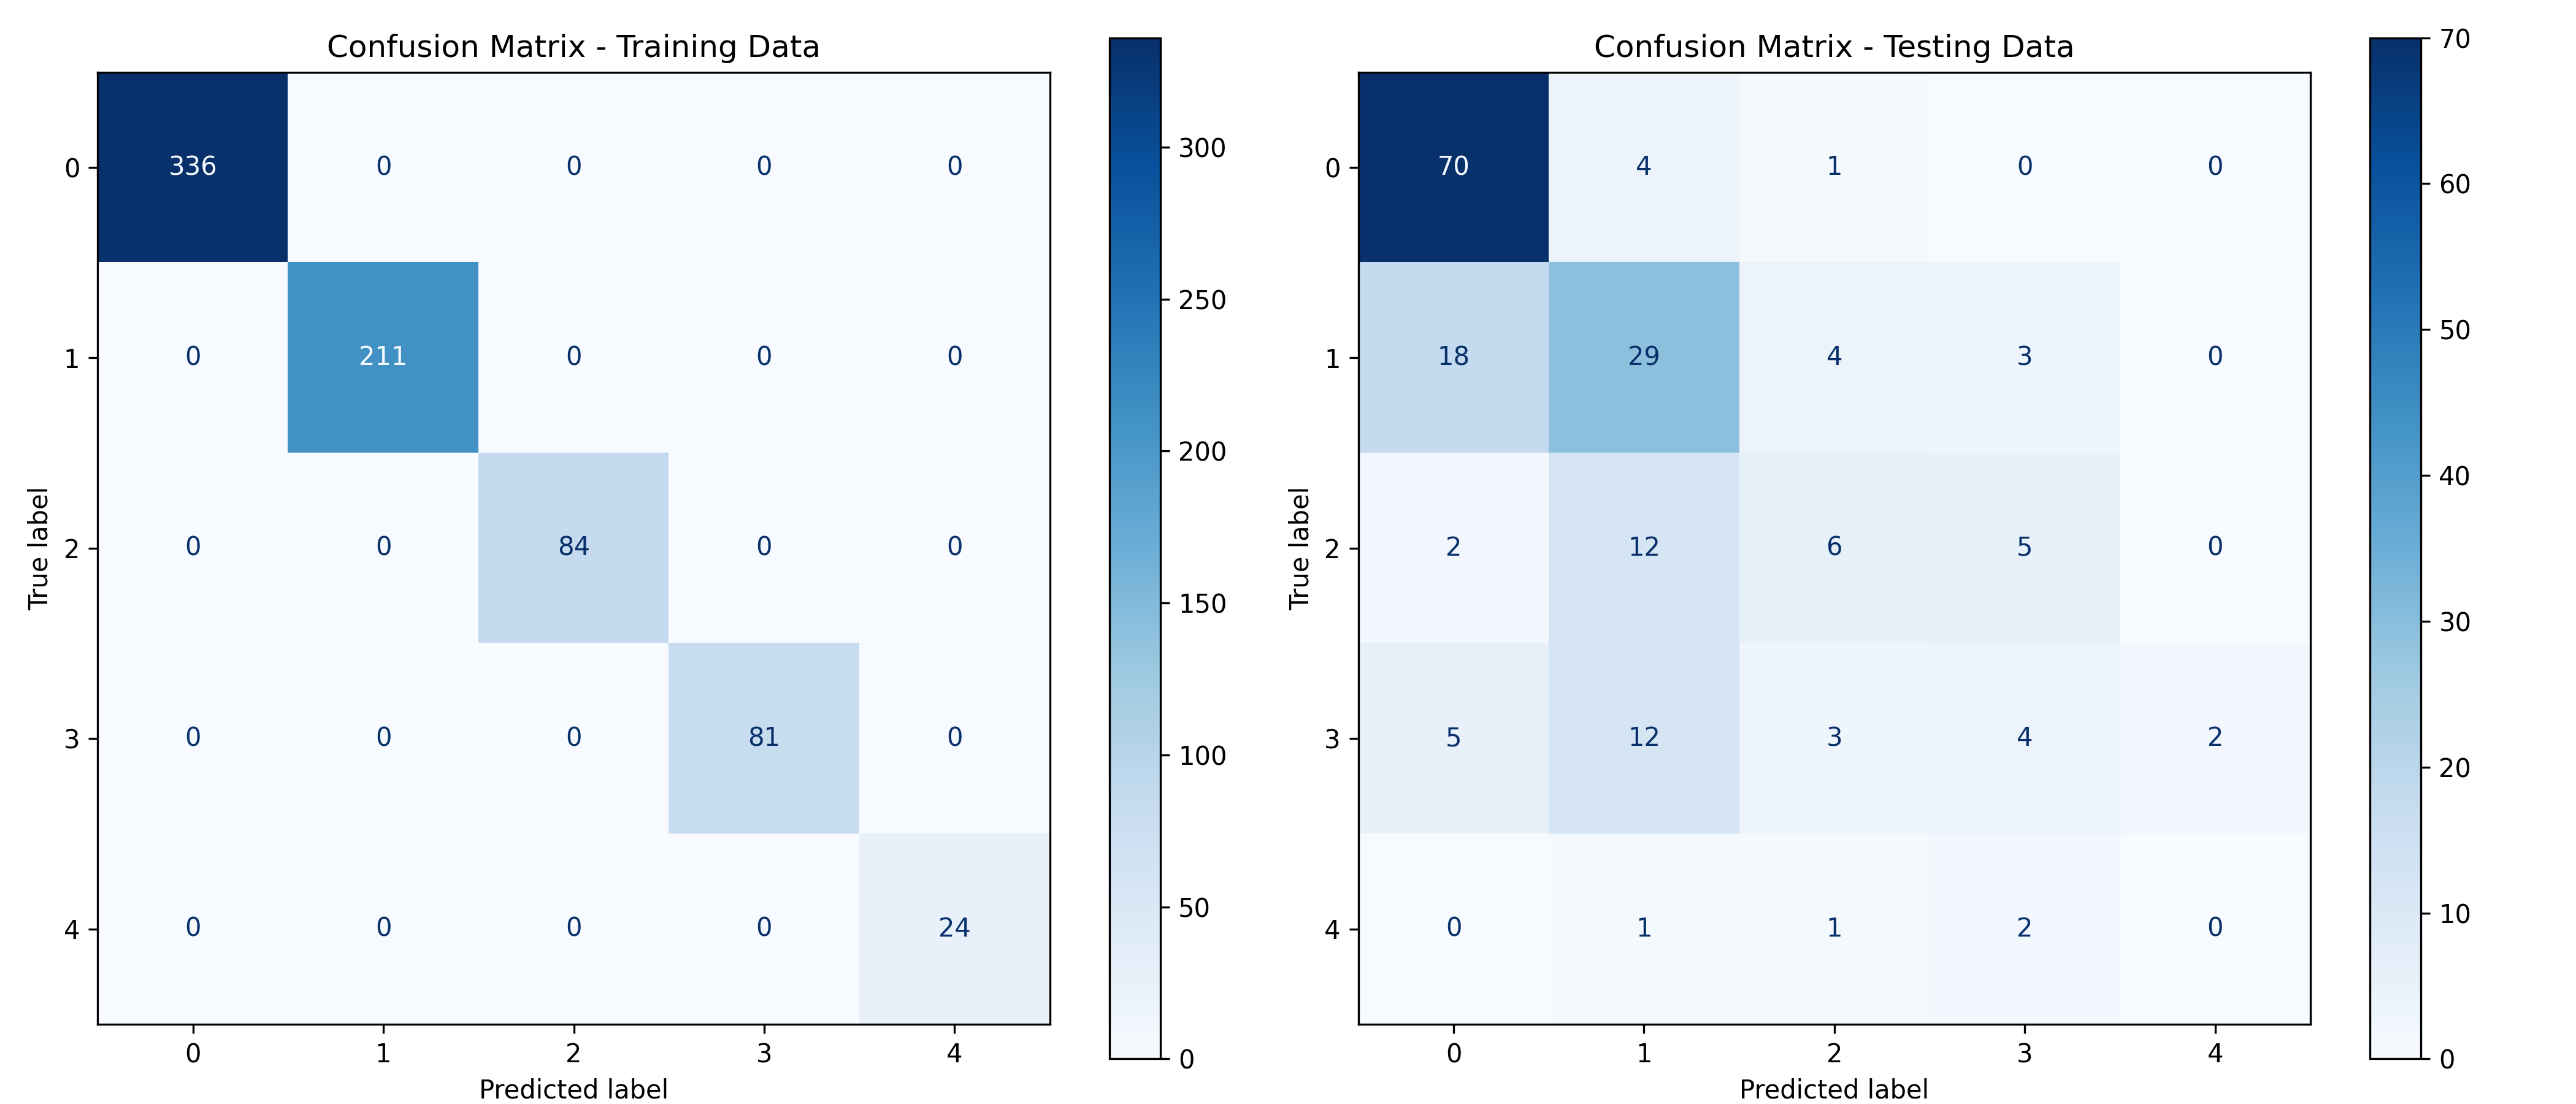
\includegraphics[width=\linewidth]{files/random1.png}
    \subcaption{Random Forest Classifier}
    \label{fig:image6}
\end{minipage}

\vspace{1em}

\begin{minipage}{0.45\textwidth}
    \centering
    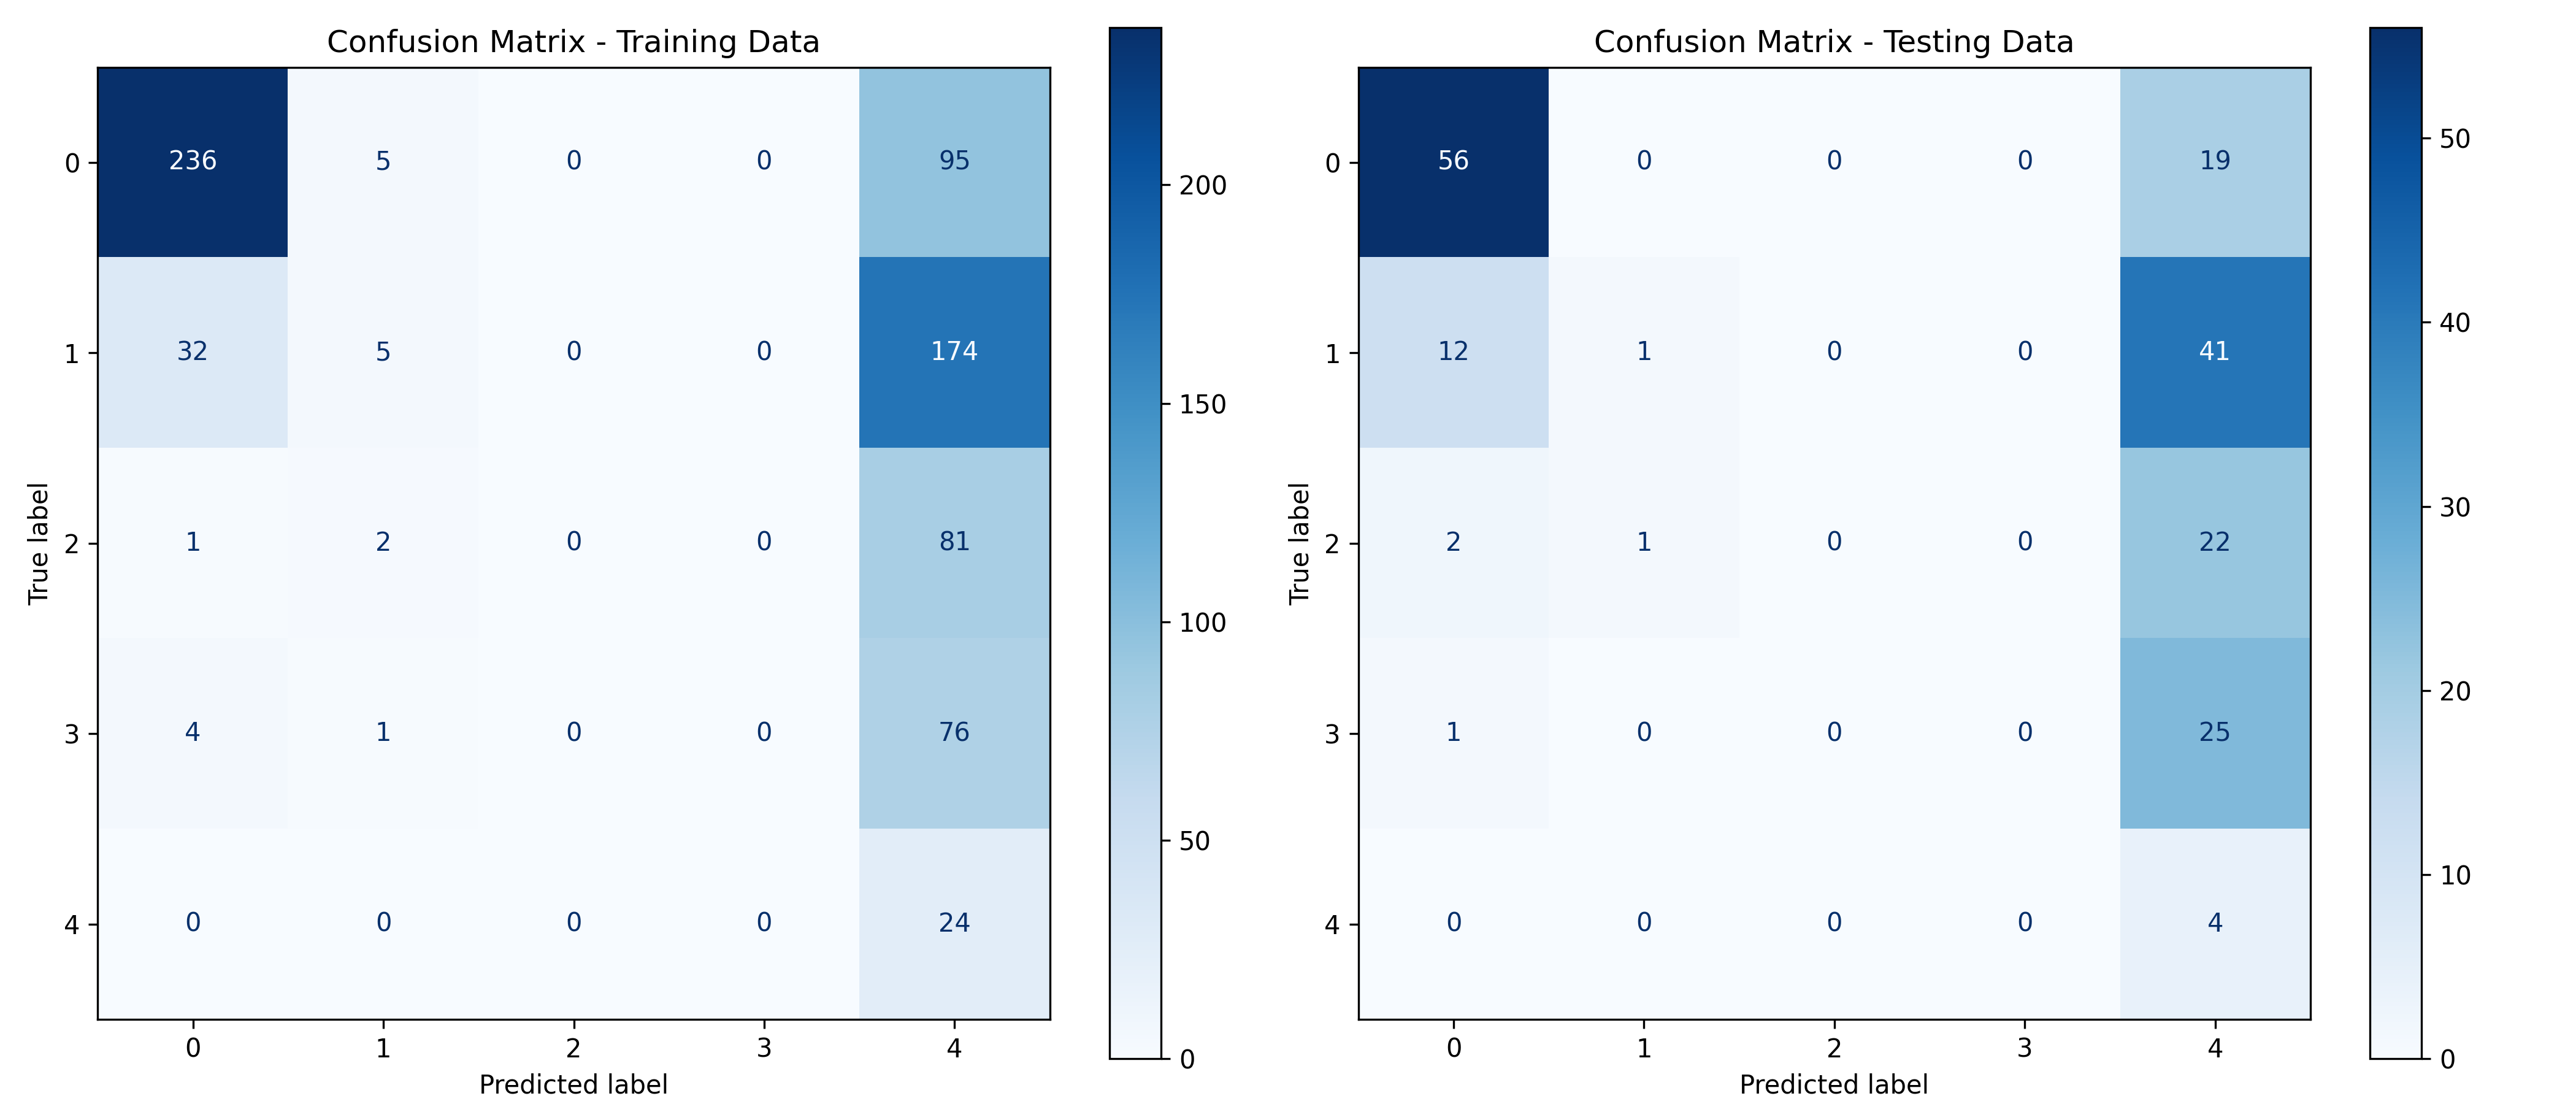
\includegraphics[width=\linewidth]{files/gau1.png}
    \subcaption{Gaussian Naive Bayes Classifier}
    \label{fig:image7}
\end{minipage}%
\hfill
\begin{minipage}{0.45\textwidth}
    \centering
    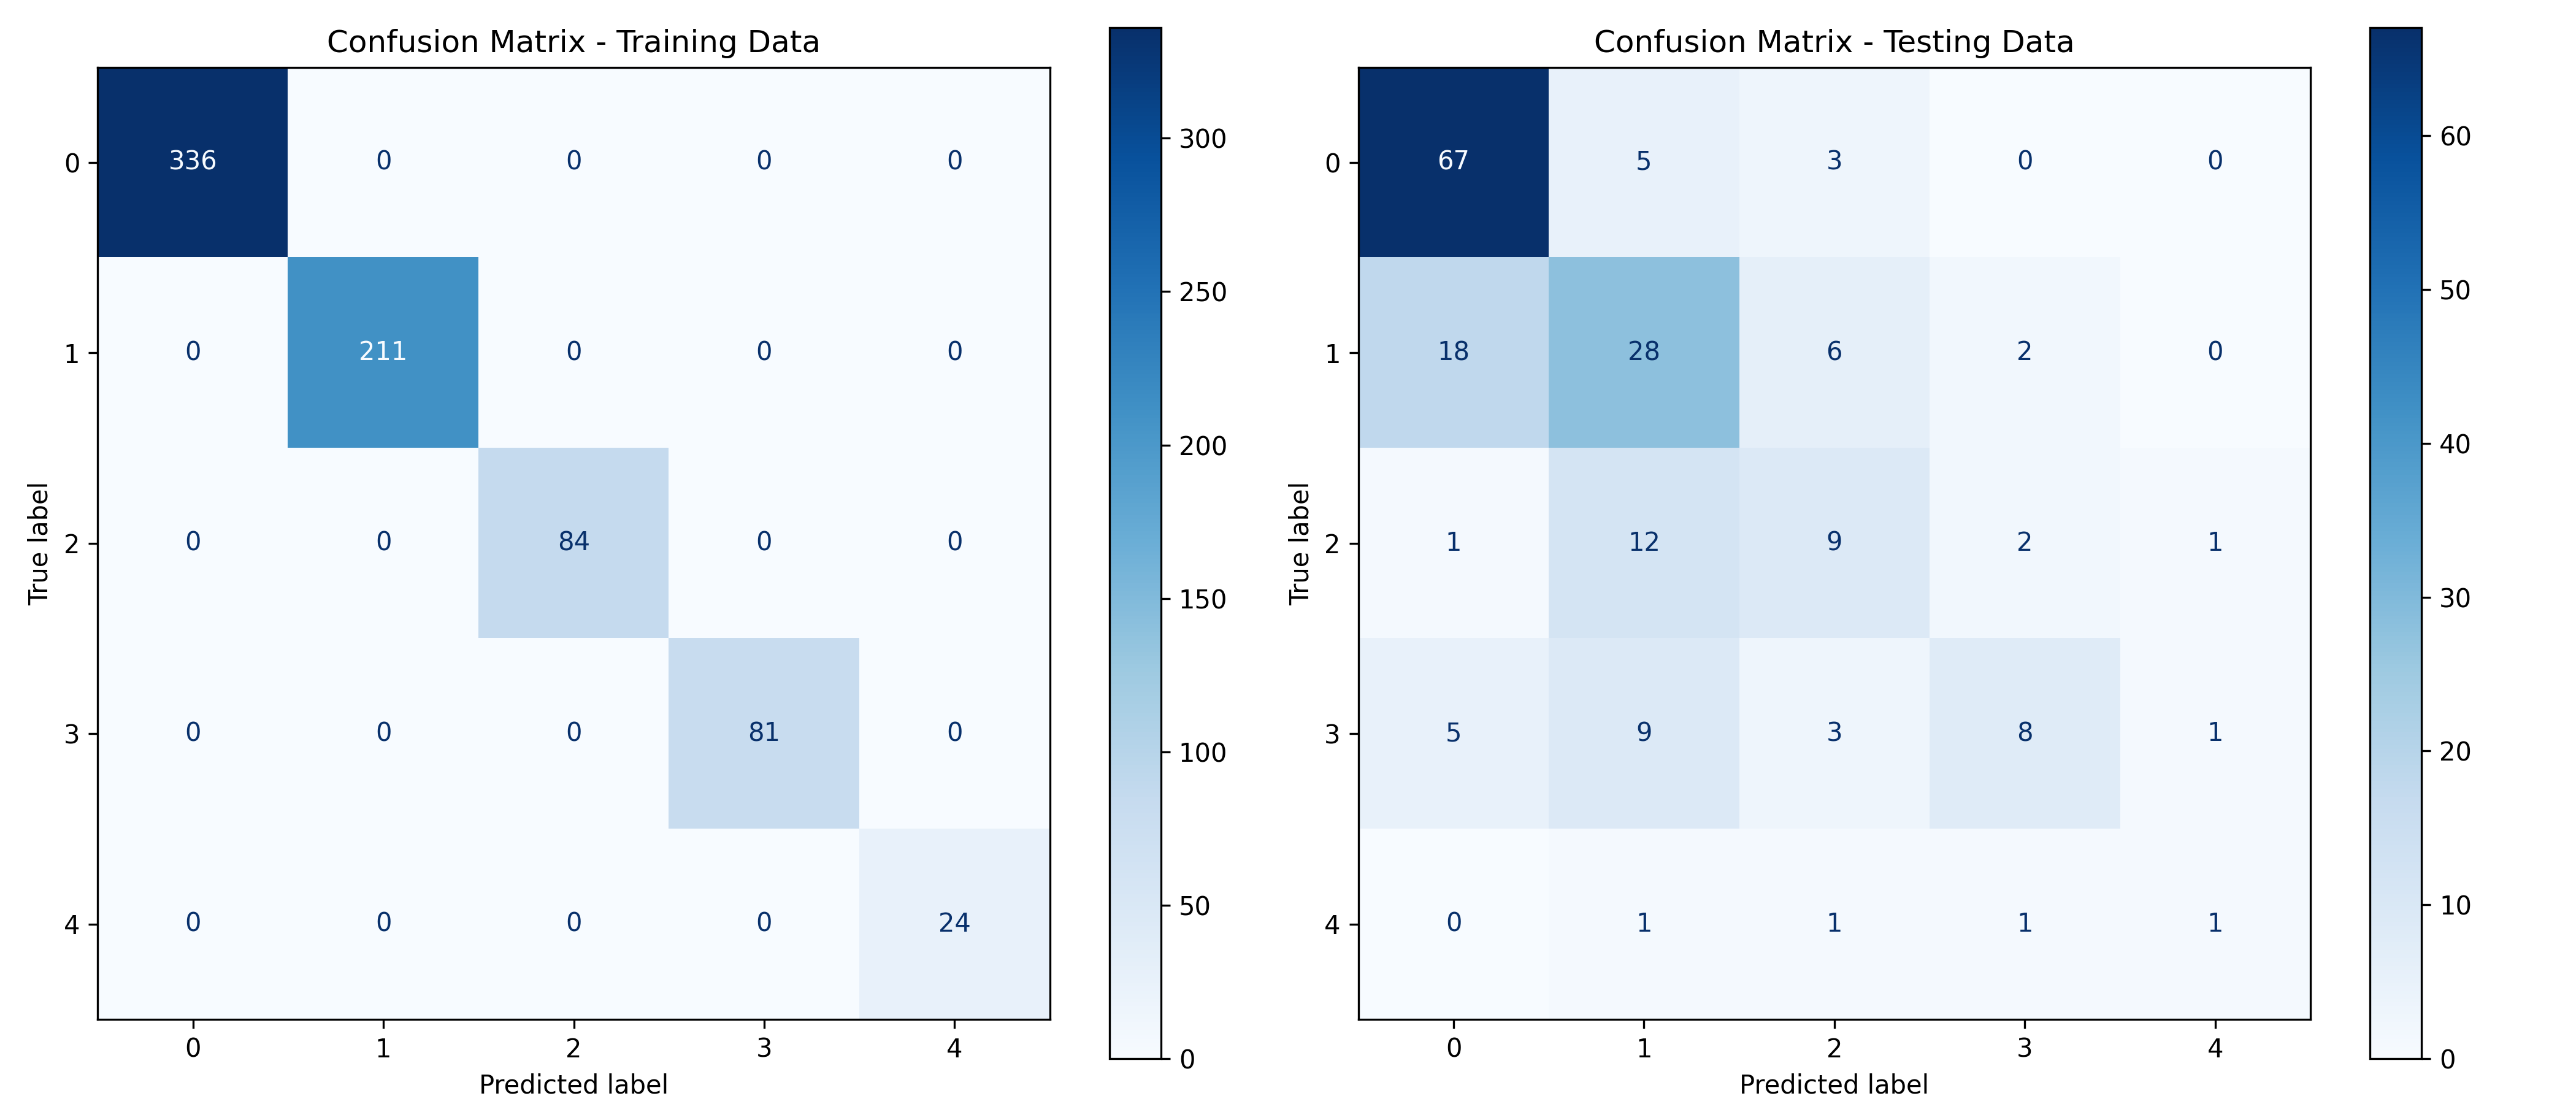
\includegraphics[width=\linewidth]{files/xgb1.png}
    \subcaption{XGBoost Classifier}
    \label{fig:image8}
\end{minipage}

\caption{Confusion Matrix for all Models}
\end{figure}


The choice of the best model depends on the specific priorities of the task at hand. For applications where accuracy is the primary concern, Gradient Boosting, Random Forest, and XGBoost are the strongest contenders. On the other hand, if interpretability is a key requirement, the Decision Tree model, despite slightly lower accuracy, may be preferred. It is important to note that this evaluation is based primarily on confusion matrices. To gain a more comprehensive understanding of model performance, we recommend incorporating additional metrics, such as precision, recall, and F1-score. Furthermore, a thorough check for overfitting, by comparing the models' performance on both training and test data, is essential to ensure the robustness of the selected model.



\textbf{model performance:} \\
The performance of various machine learning models for predicting heart disease was evaluated using metrics such as accuracy, precision, recall, F1-score, and Root Mean Square Error (RMSE). Each model’s performance is summarized below.

The K-Nearest Neighbors (KNN) model demonstrated high accuracy on both training and testing datasets, highlighting its strong overall performance. It exhibited high precision, making relatively few false positive predictions. However, its recall was slightly lower, indicating that some positive cases were missed. The F1-score was high, showing a good balance between precision and recall. Additionally, its low RMSE suggested that the predictions were close to actual values, further confirming its reliability.

Similarly, the Support Vector Machine (SVM) model achieved strong performance across all metrics. It performed comparably to KNN, handling the complexities of the dataset effectively. With high accuracy, precision, recall, and F1-score, along with a low RMSE, SVM proved to be a robust classifier for the task.

The Logistic Regression model also showcased competitive performance. It achieved metrics similar to those of KNN and SVM, with high accuracy, precision, recall, and F1-score. Its low RMSE underscored its reliability, making it a robust and interpretable choice for predicting heart disease.

The Gradient Boosting Classifier emerged as one of the top-performing models, delivering exceptional results across all evaluation metrics. Its high accuracy, precision, recall, and F1-score highlighted its capability to capture complex patterns in the data. With a very low RMSE, it stood out as a highly effective model for this problem.

The Decision Tree Classifier performed well but was slightly less accurate than other models like Gradient Boosting or Random Forest. Although it achieved high accuracy, its precision and recall were comparatively lower, resulting in a modest F1-score. This suggests that the model might have made more errors in certain cases, yet its simplicity and interpretability remain advantageous.

The Random Forest Classifier, an ensemble of decision trees, demonstrated outstanding performance, comparable to Gradient Boosting. It achieved high accuracy, precision, recall, and F1-score, along with a low RMSE. Its ability to combine the strengths of multiple trees ensured robust predictions, making it a top contender.

The Gaussian Naive Bayes model performed reasonably well, achieving high accuracy and precision. However, its recall and F1-score were relatively lower, indicating some difficulty in identifying all positive cases. This performance can be attributed to the model’s assumption of feature independence, which may not hold true for the dataset.

Finally, the XGBoost Classifier, another gradient boosting algorithm, delivered remarkable performance. It matched Gradient Boosting in accuracy, precision, recall, and F1-score while achieving a very low RMSE. Its advanced features, such as regularization, allowed it to capture complex patterns effectively, solidifying its position as one of the top-performing models.

This \autoref{table:train_per} shows the performance on the \textbf{Training Dataset} and the \autoref{table:test_per} shows the performance on \textbf{Testing dataset}

\begin{table}[h] 
\csvautotabular{files/train_per1.csv} %define this function
\caption{Training Performance}  % Table heading
\label{table:train_per}
\end{table}

\begin{table}[h] 
\csvautotabular{files/test_per2.csv} %define this function
\caption{Testing Performance}  % Table heading
\label{table:test_per}
\end{table}



 Gradient Boosting, Random Forest, and XGBoost emerged as the best models, achieving exceptional results across all metrics. KNN, SVM, and Logistic Regression also performed well and demonstrated their reliability. Decision Tree and Naive Bayes, while slightly less accurate, provided valuable insights. The selection of the most suitable model depends on the priorities of the task. For instance, models like Gradient Boosting and Random Forest would be ideal for maximizing recall, while Logistic Regression offers a simpler and more interpretable alternative.


The Decision Tree model performed exceptionally well on all metrics, achieving perfect scores (1.00 for accuracy, precision, recall, and F1-score) and zero errors (0.00 RMSE). This suggests that the model is highly effective at classifying the data and predicting both the positive and negative classes correctly. However, it's crucial to ensure that the dataset used is not overly simplified or imbalanced, as perfect scores can sometimes be a result of overfitting, especially in small datasets. It may also be beneficial to cross-validate the model with different datasets to ensure its generalizability. The Decision Tree model shows outstanding performance across key evaluation metrics, making it a strong candidate for the classification task at hand, assuming the dataset is representative and appropriately balanced \autoref{table:train_best}.

\begin{table}[h] 
\csvautotabular{files/best_train.csv} %define this function
\caption{Best Model on Training Dataset}  % Table heading
\label{table:train_best}
\end{table}

XGBoost emerged as the best model in terms of accuracy, precision, recall, and F1-Score, making it the top choice for classification tasks in this project. However, its scores indicate moderate performance, suggesting that further optimization, such as feature engineering, hyperparameter tuning, or adding more data, is needed.
Gradient Boosting performed better in terms of RMSE, which, although not a primary metric for classification, reflects the model's stability in prediction. It might be worth exploring its performance further for tasks requiring consistent predictions \autoref{table:test_best}.

\begin{table}[h] 
\csvautotabular{files/best_test.csv} %define this function
\caption{Best Model on Testing Dataset}  % Table heading
\label{table:test_best}
\end{table}

\section{Performance Analysis of Machine Learning Models}

This section presents a detailed performance analysis of several machine learning algorithms based on various evaluation metrics. These metrics include execution time, classification accuracy, precision for both "YES" and "NO" classes, the Kappa statistic, Mean Absolute Error (MAE), and the percentage of correctly and incorrectly classified instances \autoref{table:result}.

\subsection{Execution Time}
The execution time for each algorithm varies significantly. The \textbf{K-Nearest Neighbors (KNN)} algorithm is the fastest, taking only 0.008533 seconds, which is expected since KNN does not involve complex training and performs most of the computation during testing. Conversely, \textbf{Gradient Boosting} and \textbf{Naive Bayes} take significantly longer at 1.314636 and 1.148516 seconds, respectively. \textbf{Gradient Boosting} is computationally intensive because it builds multiple sequential trees, while the long runtime for \textbf{Naive Bayes} might be due to data preprocessing overhead or inefficiencies in its implementation. \textbf{XGBoost}, an optimized boosting method, has a moderate runtime of 0.409072 seconds, balancing efficiency and complexity. While time is crucial in applications requiring real-time predictions, algorithms like \textbf{Gradient Boosting} and \textbf{XGBoost} may still be viable when accuracy is prioritized over speed.

\subsection{Classification Accuracy and Error}
The percentage of correctly classified instances is a primary indicator of the model's effectiveness. \textbf{XGBoost} outperforms all other models, correctly classifying 61.41\% of instances, followed closely by \textbf{Gradient Boosting} with 60.33\% \autoref{table:result}. This demonstrates the power of boosting techniques in capturing complex relationships within the dataset. On the other hand, \textbf{Naive Bayes} has the lowest classification accuracy at 33.15\%, highlighting its limitations. The high incorrectly classified percentage (66.85\%) for \textbf{Naive Bayes} shows that its strong assumption of feature independence does not align well with the dataset's characteristics. In contrast, the lower error rates for \textbf{XGBoost} (38.59\%) and \textbf{Gradient Boosting} (39.67\%) make them more reliable for practical applications.

\subsection{Kappa Statistic}
The \textbf{Kappa statistic} measures the agreement between predicted and actual values while accounting for the possibility of agreement occurring by chance \autoref{table:result}. \textbf{XGBoost} achieves the highest Kappa score of 0.4359, indicating moderate agreement and solid performance. \textbf{Gradient Boosting} follows closely with a score of 0.4142. These values suggest that these models capture the underlying patterns of the data effectively. Conversely, \textbf{Naive Bayes} has the lowest Kappa score of 0.1911, reflecting poor agreement and further emphasizing its inability to model the dataset effectively. Models with higher Kappa statistics, like \textbf{XGBoost}, are more dependable for making predictions.

\subsection{Mean Absolute Error (MAE)}
MAE represents the average magnitude of errors in predictions, regardless of direction. Models with lower MAE values make predictions that are closer to the true values. Both \textbf{Gradient Boosting} and \textbf{XGBoost} achieve the lowest MAE of 0.5434, reinforcing their reliability in this dataset. In contrast, \textbf{Naive Bayes} has a significantly higher MAE of 1.5652, indicating that its predictions deviate substantially from the true labels. This metric confirms the superior accuracy of ensemble models like \textbf{XGBoost} and \textbf{Gradient Boosting} compared to simpler models like \textbf{Naive Bayes}.

\subsection{Precision for "YES" and "NO" Classes}
Precision measures the proportion of true positive predictions out of all positive predictions. For the "YES" class, \textbf{XGBoost} achieves the highest precision at 0.5206, followed by \textbf{Gradient Boosting} at 0.4475. This indicates that these models are effective at minimizing false positives when predicting the positive class. Similarly, \textbf{XGBoost} and \textbf{Gradient Boosting} excel in precision for the "NO" class, reflecting their balanced performance across both classes. On the other hand, \textbf{Naive Bayes} struggles with precision for both classes, achieving the lowest values of 0.2649, making it unsuitable for applications where minimizing false positives is critical \autoref{table:result}.

\subsection{Classification Categories}
The algorithms are grouped into four categories: \textbf{Functions}, \textbf{Boosting}, \textbf{Trees}, and \textbf{Bayes}. Models under the \textbf{Boosting} category, such as \textbf{Gradient Boosting} and \textbf{XGBoost}, show superior performance due to their iterative approach, where each model learns from the errors of the previous one. \textbf{Tree-based} models, like \textbf{Random Forest} and \textbf{Decision Tree}, perform moderately well but fall short of the boosting methods. Models categorized as \textbf{Functions}, including \textbf{KNN}, \textbf{SVM}, and \textbf{Logistic Regression}, exhibit average performance. Finally, the \textbf{Bayes} category, represented by \textbf{Naive Bayes}, is the weakest performer due to its unrealistic assumption that features are independent, which does not hold true for this dataset \autoref{table:result}.



This analysis from \autoref{table:result} highlights the strengths of ensemble methods, particularly \textbf{XGBoost} and \textbf{Gradient Boosting}, in handling complex datasets. Their ability to build robust models through iterative learning makes them the most suitable choices for this dataset. Simpler models like \textbf{KNN}, \textbf{SVM}, and \textbf{Logistic Regression} provide average performance but are outperformed by ensemble techniques. \textbf{Naive Bayes}, although fast, fails to provide reliable predictions due to its unrealistic assumptions. Based on the results, \textbf{XGBoost} and \textbf{Gradient Boosting} should be prioritized in applications requiring high accuracy and balanced predictions. The final choice of the model should also consider the computational constraints and the specific requirements of the application \autoref{table:result}.


\begin{table}[ht]
\centering
\hspace*{-1.5cm} % Shift table to the left (-1.5cm can be adjusted)
\resizebox{1.2\textwidth}{!}{ % Resize table to exceed normal width
\begin{tabular}{lcccccccccc}
\toprule
Algorithm & Time & \% Correct & \% Incorrect & Attributes & Instances & Kappa & MAE & Prec. YES & Prec. NO \\
\midrule
KNN & 0.01 & 56.52 & 43.48 & 16 & 920 & 0.35 & 0.64 & 0.34 & 0.34 \\
SVM & 0.07 & 53.8 & 46.2 & 16 & 920 & 0.3 & 0.66 & 0.31 & 0.31 \\
Log. Reg. & 0.03 & 54.89 & 45.11 & 16 & 920 & 0.33 & 0.61 & 0.32 & 0.32 \\
Gradient Boosting & 1.31 & 60.33 & 39.67 & 16 & 920 & 0.41 & 0.54 & 0.45 & 0.45 \\
Decision Tree & 0.01 & 55.43 & 44.57 & 16 & 920 & 0.37 & 0.62 & 0.41 & 0.41 \\
Random Forest & 0.27 & 59.24 & 40.76 & 16 & 920 & 0.4 & 0.58 & 0.38 & 0.38 \\
Naive Bayes & 1.15 & 33.15 & 66.85 & 16 & 920 & 0.19 & 1.57 & 0.26 & 0.26 \\
XGBoost & 0.41 & 61.41 & 38.59 & 16 & 920 & 0.44 & 0.54 & 0.52 & 0.52 \\
\bottomrule
\end{tabular}
}
\caption{Performance Comparison between all Machine Learning Models}
\label{table:result}

\end{table}

\section{Discussion}

\subsection{Interpretation of Results and Their Significance}
The study evaluated various machine learning algorithms to classify heart disease risk using the UCI Heart Disease dataset. Among the tested models, ensemble methods such as Gradient Boosting, Random Forest, and XGBoost consistently outperformed others in terms of accuracy, precision, recall, and F1-score, with XGBoost emerging as the top-performing model during testing (accuracy: 61.41\%, F1-score: 0.60). These results underline the effectiveness of ensemble techniques in capturing complex, non-linear relationships in medical data.

The superior performance of Gradient Boosting and XGBoost demonstrates their ability to generalize well, even in datasets with overlapping class distributions and imbalanced data. Conversely, simpler models like Logistic Regression and KNN exhibited moderate performance, highlighting their limitations in handling intricate feature interactions present in medical datasets. The Decision Tree model, while interpretable and achieving high training scores, was prone to overfitting, underscoring the importance of regularization mechanisms in tree-based models. The findings suggest that ensemble methods are well-suited for clinical decision support systems where accurate predictions are crucial.

\subsection{Addressing Anomalies or Unexpected Findings}
\begin{itemize}
    \item \textbf{Perfect Training Scores with Decision Tree and Random Forest Models:} Both models achieved perfect accuracy, precision, recall, and F1-scores during training, which is indicative of overfitting. The testing performance of these models dropped significantly, confirming the hypothesis. This highlights a need for hyperparameter tuning and cross-validation to prevent overfitting in future implementations.
    \item \textbf{Naive Bayes' Poor Performance:} Naive Bayes significantly underperformed, with an accuracy of 33.15\% and a high RMSE of 1.57. This likely stems from its assumption of feature independence, which is unrealistic for this dataset. Medical data typically involve correlated features (e.g., cholesterol and blood pressure), which the Naive Bayes model fails to account for.
    \item \textbf{Gradient Boosting's Computational Demand:} While Gradient Boosting demonstrated strong predictive performance, it required the longest execution time (1.31 seconds). This may limit its utility in real-time applications unless computational resources are optimized.
    \item \textbf{Moderate Performance of SVM:} Despite its theoretical strength in high-dimensional spaces, SVM exhibited suboptimal performance with an accuracy of 54\%. This might result from a lack of tuning or the kernel selection not aligning well with the dataset's characteristics.
\end{itemize}

\section{Conclusion}
This study explored the application of machine learning techniques to predict heart disease risk using the UCI Heart Disease dataset, evaluating nine models. Ensemble methods, particularly Gradient Boosting, Random Forest, and XGBoost, consistently outperformed other models, excelling in accuracy, precision, recall, and F1-score. XGBoost, in particular, was identified as the top-performing model due to its robustness and scalability. The research highlighted the strengths of ensemble learning in medical diagnostics but also underscored the limitations of simpler algorithms like Naive Bayes, which struggled due to unrealistic assumptions, and Decision Trees, which tended to overfit. The study achieved its objectives of implementing and comparing multiple models, ensuring high-quality input data, and identifying the best-performing algorithms. Future research could focus on addressing data imbalance, hyperparameter optimization, enhanced feature engineering, model interpretability, scalability to real-world applications, and the integration of temporal data for dynamic risk assessments.

\pagebreak
\section*{Acknowledgments}

We would like to express our sincere gratitude to our supervisor, \textbf{\href{https://cs.rkmvu.ac.in/~tamal/}{Br. Tamal}} (\href{tamal@gm.rkmvu.ac.in}{email}), Assistant Professor in the Department of Computer Science at RKMVERI, for his invaluable guidance, encouragement, and support throughout the course of this project. His expertise in machine learning and his insightful suggestions were instrumental in shaping this research.

We would also like to thank \textbf{\href{cs.rkmvu.ac.in}{Ramakrishna Mission Vivekananda Educational and Research Institute}} for providing the necessary resources and facilities that enabled the successful completion of this project.

Lastly, we extend our heartfelt thanks to our batch mates for their constant encouragement and understanding during the challenging phases of this project.
\pagebreak


% \pagebreak
\bibliography{sn-bibliography}% common bib file
%% if required, the content of .bbl file can be included here once bbl is generated
%%\input sn-article.bbl


\end{document}
